% ============================================================
%  TD5: SVM, Random Forest y Datos Desbalanceados
%  Curso: Machine Learning Industrial
% ============================================================
\documentclass[12pt,a4paper]{article}

% --- Paquetes ---
\usepackage[T1]{fontenc}
\usepackage[utf8]{inputenc}
\usepackage[spanish]{babel}
\usepackage[top=2.5cm, bottom=2.5cm, left=2.8cm, right=2.8cm, headheight=14pt]{geometry}
\usepackage{amsmath, amssymb}
\usepackage{booktabs}
\usepackage{graphicx}
\usepackage{float}
\usepackage{xcolor}
\usepackage{listings}
\usepackage{hyperref}
\usepackage{parskip}
\usepackage{titlesec}
\usepackage{enumitem}
\usepackage{array}
\usepackage{colortbl}
\usepackage{multirow}
\usepackage{fancyhdr}
\usepackage{mdframed}
\usepackage{tcolorbox}
\usepackage{subcaption}

% --- Ruta de imagenes ---
\graphicspath{{img/}}

% --- Colores corporativos ---
\definecolor{azulTDS}{RGB}{0, 70, 127}
\definecolor{verdeTDS}{RGB}{0, 120, 80}
\definecolor{grisClaro}{RGB}{245, 245, 245}
\definecolor{grisMedio}{RGB}{200, 200, 200}
\definecolor{rojoPeligro}{RGB}{180, 30, 30}
\definecolor{naranjaPorque}{RGB}{255, 140, 0}
\definecolor{azulPorque}{RGB}{0, 100, 180}
\definecolor{codebg}{RGB}{248, 248, 248}
\definecolor{codeframe}{RGB}{180, 180, 200}
\definecolor{keywordcolor}{RGB}{0, 80, 160}
\definecolor{commentcolor}{RGB}{80, 130, 80}
\definecolor{stringcolor}{RGB}{160, 40, 40}

% --- Configuracion de listings (codigo Python) ---
\lstset{
  language=Python,
  basicstyle=\ttfamily\small,
  keywordstyle=\bfseries\color{keywordcolor},
  commentstyle=\itshape\color{commentcolor},
  stringstyle=\color{stringcolor},
  backgroundcolor=\color{codebg},
  frame=single,
  framerule=0.6pt,
  rulecolor=\color{codeframe},
  numbers=left,
  numberstyle=\tiny\color{gray},
  numbersep=6pt,
  breaklines=true,
  breakatwhitespace=false,
  showstringspaces=false,
  tabsize=4,
  captionpos=b,
  xleftmargin=1.5em,
  framexleftmargin=1.5em,
}

% --- Encabezado y pie de pagina ---
\pagestyle{fancy}
\fancyhf{}
\fancyhead[L]{\small\textcolor{azulTDS}{\textbf{TD5 -- Machine Learning Industrial}}}
\fancyhead[R]{\small\textcolor{azulTDS}{SVM, Random Forest y Datos Desbalanceados}}
\fancyfoot[C]{\small\thepage}
\renewcommand{\headrulewidth}{0.4pt}
\renewcommand{\footrulewidth}{0.2pt}

% --- Formato de secciones ---
\titleformat{\section}[block]
  {\Large\bfseries\color{azulTDS}}
  {\thesection.}{0.5em}{}
  [\vspace{-0.3em}\rule{\textwidth}{1.5pt}]

\titleformat{\subsection}[block]
  {\large\bfseries\color{verdeTDS}}
  {\thesubsection.}{0.5em}{}

\titleformat{\subsubsection}[block]
  {\normalsize\bfseries\color{black}}
  {\thesubsubsection.}{0.5em}{}

% --- Cajas de resultados ---
\tcbuselibrary{skins, breakable}
\tcbset{
  resultbox/.style={
    colback=grisClaro,
    colframe=azulTDS,
    fonttitle=\bfseries,
    title={Resultado},
    left=4pt, right=4pt, top=4pt, bottom=4pt,
    breakable
  },
  warnbox/.style={
    colback=yellow!8,
    colframe=rojoPeligro,
    fonttitle=\bfseries\color{rojoPeligro},
    title={Punto clave},
    left=4pt, right=4pt, top=4pt, bottom=4pt,
    breakable
  },
  codebox/.style={
    colback=codebg,
    colframe=codeframe,
    fonttitle=\bfseries,
    left=4pt, right=4pt, top=4pt, bottom=4pt,
    breakable
  },
  porquebox/.style={
    colback=azulPorque!8,
    colframe=azulPorque,
    fonttitle=\bfseries\color{azulPorque},
    title={Por que este paso?},
    left=6pt, right=6pt, top=6pt, bottom=6pt,
    breakable
  }
}

% --- Comando para caja "Por que" simple ---
\newcommand{\porqueRule}[1]{%
  \vspace{4pt}%
  \noindent\rule{\textwidth}{0.6pt}\\[2pt]%
  \textbf{\textcolor{azulPorque}{Por que este paso?}}\quad #1\\[2pt]%
  \noindent\rule{\textwidth}{0.6pt}%
  \vspace{4pt}%
}

% --- Hiperreferencias ---
\hypersetup{
  colorlinks=true,
  linkcolor=azulTDS,
  urlcolor=verdeTDS,
  citecolor=azulTDS,
  pdftitle={TD5: SVM, Random Forest y Datos Desbalanceados},
  pdfauthor={Machine Learning Industrial},
}

% ============================================================
\begin{document}
% ============================================================

% ---- PORTADA -----------------------------------------------
\begin{titlepage}
  \centering
  \vspace*{2cm}

  {\Huge\bfseries\color{azulTDS}
    Trabajo Dirigido 5 (TD5)\\[0.6em]
    \rule{0.8\textwidth}{2pt}\\[0.6em]
    SVM, Random Forest\\y Datos Desbalanceados
  }

  \vspace{1.5cm}
  {\Large\bfseries\color{verdeTDS} Curso de Machine Learning Industrial}

  \vspace{0.8cm}
  {\large Mantenimiento Predictivo con Aprendizaje Supervisado}

  \vspace{2.5cm}

  \begin{tcolorbox}[colback=azulTDS!8, colframe=azulTDS, width=0.82\textwidth,
      left=12pt, right=12pt, top=10pt, bottom=10pt]
    \centering
    \begin{tabular}{ll}
      \textbf{Tema:}       & SVM, Random Forest, Desbalance de Clases \\[4pt]
      \textbf{Herramientas:} & Python, scikit-learn, imbalanced-learn   \\[4pt]
      \textbf{Dataset:}    & \texttt{make\_moons}, \texttt{make\_classification} \\[4pt]
      \textbf{Fecha:}      & Junio 2026                               \\[4pt]
      \textbf{Ejercicios:} & 3 ejercicios, 12 preguntas               \\
    \end{tabular}
  \end{tcolorbox}

  \vspace{2.5cm}

  {\large\itshape
    ``El conocimiento de los algoritmos de clasificacion y el manejo correcto\\
    de datos desbalanceados son pilares fundamentales del\\
    mantenimiento predictivo industrial basado en datos.''
  }

  \vfill
  {\small\color{gray} Machine Learning Industrial --- TD5 --- 2026}
\end{titlepage}

% ---- TABLA DE CONTENIDOS -----------------------------------
\tableofcontents
\newpage

% ============================================================
% RESUMEN EJECUTIVO
% ============================================================
\section*{Resumen Ejecutivo}
\addcontentsline{toc}{section}{Resumen Ejecutivo}

Este documento presenta el desarrollo completo del Trabajo Dirigido 5 (TD5) del curso de Machine Learning Industrial. El TD5 aborda tres grandes bloques tematicos fundamentales para el mantenimiento predictivo:

\begin{enumerate}[label=\textbf{\arabic*.}]
  \item \textbf{Support Vector Machines (SVM):} Se estudia la clasificacion de un dataset no linealmente separable (\texttt{make\_moons}) con kernels lineal, RBF y polinomial. Se realiza optimizacion de hiperparametros mediante \texttt{GridSearchCV} y se compara con regresion logistica.

  \item \textbf{Random Forest (RF):} Se exploran los efectos del numero de arboles (\texttt{n\_estimators}) y la profundidad maxima (\texttt{max\_depth}) sobre el rendimiento. Se analiza el sobreajuste (overfitting), las importancias de variables y se compara con un arbol de decision unico.

  \item \textbf{Manejo de Datasets Desbalanceados:} Con un ratio 90\%/10\% (Normal/Fallo), se estudia por que la exactitud (accuracy) es una metrica enganosa, y se comparan tres estrategias de correccion: pesos de clase (\texttt{class\_weight}), sobremuestreo sintetico (SMOTE) y submuestreo aleatorio.
\end{enumerate}

\begin{tcolorbox}[resultbox, title={Resultados Destacados}]
  \begin{itemize}[leftmargin=1.5em]
    \item SVM con kernel RBF (C=10) alcanza \textbf{95\% de accuracy} en \texttt{make\_moons}, frente al 85\% de la regresion logistica lineal.
    \item Random Forest con \texttt{max\_depth=10} ofrece el mejor equilibrio bias-varianza, eliminando el overfitting total del arbol unico profundo.
    \item En datos desbalanceados (ratio 9:1), el modelo base ignora el 30\% de los fallos reales. Con pesos de clase, el recall de fallos mejora del 71\% al \textbf{90\%}.
    \item SMOTE y submuestreo aleatorio logran mejoras comparables con distintos trade-offs en tiempo de entrenamiento e informacion disponible.
  \end{itemize}
\end{tcolorbox}

\subsection*{Mapa de Figuras del Documento}

Este documento integra \textbf{14 figuras} extraidas directamente del notebook de experimentacion. La tabla siguiente describe su distribucion:

\begin{table}[H]
  \centering
  \caption{Catalogo de figuras del TD5}
  \label{tab:figuras}
  \begin{tabular}{clll}
    \toprule
    \textbf{Fig.} & \textbf{Archivo} & \textbf{Contenido} & \textbf{Ejercicio} \\
    \midrule
    1  & td5\_cell001\_img00 & Dataset make\_moons (scatter) & Ej.~1 \\
    2  & td5\_cell004\_img01 & Frontera SVM default RBF & Ej.~1 \\
    3  & td5\_cell014\_img02 & 3 fronteras SVM comparadas & Ej.~1 \\
    4  & td5\_cell019\_img03 & SVM RBF vs Regresion Logistica & Ej.~1 \\
    5  & td5\_cell025\_img04 & RF default: frontera decision & Ej.~2 \\
    6  & td5\_cell030\_img05 & Efecto n\_estimators & Ej.~2 \\
    7  & td5\_cell033\_img06 & Efecto max\_depth & Ej.~2 \\
    8  & td5\_cell038\_img07 & Feature importances (barras) & Ej.~2 \\
    9  & td5\_cell039\_img08 & 3 fronteras RF: under/best/over & Ej.~2 \\
    10 & td5\_cell043\_img09 & Dataset desbalanceado (scatter) & Ej.~3 \\
    11 & td5\_cell046\_img10 & Baseline LR: CM + frontera & Ej.~3 \\
    12 & td5\_cell051\_img11 & Class weights: 3 paneles & Ej.~3 \\
    13 & td5\_cell056\_img12 & SMOTE: 3 paneles & Ej.~3 \\
    14 & td5\_cell061\_img13 & Undersampling: 3 paneles & Ej.~3 \\
    \bottomrule
  \end{tabular}
\end{table}

\newpage

% ============================================================
% EJERCICIO 1: SVM
% ============================================================
\section{Ejercicio 1: Support Vector Machines (SVM)}

\subsection{Contexto y Motivacion Industrial}

\begin{tcolorbox}[porquebox, title={Por que SVM para mantenimiento predictivo?}]
En mantenimiento predictivo, los datos de sensores (vibracion, temperatura, corriente) rara vez
son \textit{linealmente separables}. Las condiciones de fallo emergente forman patrones no
lineales en el espacio de caracteristicas: por ejemplo, una combinacion especifica de frecuencia
de vibracion alta \textit{y} temperatura elevada puede indicar un rodamiento deteriorado, pero
ninguna de las dos variables sola es suficiente. SVM con kernel RBF puede capturar estas
interacciones no lineales sin necesidad de disenar features manualmente, proyectando los datos a
un espacio de alta dimension donde la frontera de decision si existe.
\end{tcolorbox}

Las Support Vector Machines (SVM) son clasificadores que buscan el hiperplano de maximo margen
que separa dos clases en el espacio de caracteristicas. Su potencia reside en el \textit{kernel
trick}: al proyectar implicitamente los datos a un espacio de mayor dimension, pueden encontrar
fronteras de decision no lineales sin calcular explicitamente la transformacion.

La formulacion matematica del SVM de margen suave minimiza:
\begin{equation}
  \min_{\mathbf{w}, b, \boldsymbol{\xi}} \frac{1}{2}\|\mathbf{w}\|^2 + C\sum_{i=1}^{n}\xi_i
  \quad \text{s.t.} \quad y_i(\mathbf{w}^T\phi(\mathbf{x}_i) + b) \geq 1 - \xi_i,\; \xi_i \geq 0
  \label{eq:svm_primal}
\end{equation}
donde $\phi(\mathbf{x})$ es la transformacion implicitamente definida por el kernel, $\xi_i$ son
variables de holgura, y $C$ controla el trade-off entre margen y errores de clasificacion.

\subsubsection*{Generacion del dataset}

\begin{tcolorbox}[porquebox, title={Por que make\_moons con noise=0.25?}]
\texttt{make\_moons} genera dos semicircunferencias entrelazadas que son \textit{imposibles de
separar con una linea recta}. Es el dataset canonico para demostrar la necesidad de kernels no
lineales. El parametro \texttt{noise=0.25} introduce dispersion gaussiana que simula la
variabilidad de sensores reales, haciendo el problema mas parecido a situaciones industriales
donde los datos de entrenamiento son ruidosos.
\end{tcolorbox}

\begin{lstlisting}[caption={Generacion y preparacion del dataset make\_moons}]
from sklearn.datasets import make_moons
from sklearn.model_selection import train_test_split

X, y = make_moons(n_samples=500, noise=0.25, random_state=42)
X_train, X_test, y_train, y_test = train_test_split(
    X, y, test_size=0.2, random_state=42
)

# Las columnas representan:
# X[:,0] -> Vibration_Frequency (frecuencia de vibracion)
# X[:,1] -> Temperature_Index   (indice de temperatura)
\end{lstlisting}

El dataset \textbf{\texttt{make\_moons}} genera dos nubes de puntos en forma de medias lunas
entrelazadas. La distribucion resultante tiene las siguientes caracteristicas:
\begin{itemize}
  \item \textbf{500 muestras} totales (400 entrenamiento, 100 test)
  \item \textbf{2 features} continuas: \texttt{Vibration\_Frequency} y \texttt{Temperature\_Index}
  \item \textbf{2 clases} perfectamente balanceadas (250 cada una)
  \item \textbf{No separable linealmente}: ningun hiperplano puede separar ambas clases con baja tasa de error
\end{itemize}

% --- FIGURA 1: Dataset make_moons ---
\begin{figure}[H]
  \centering
  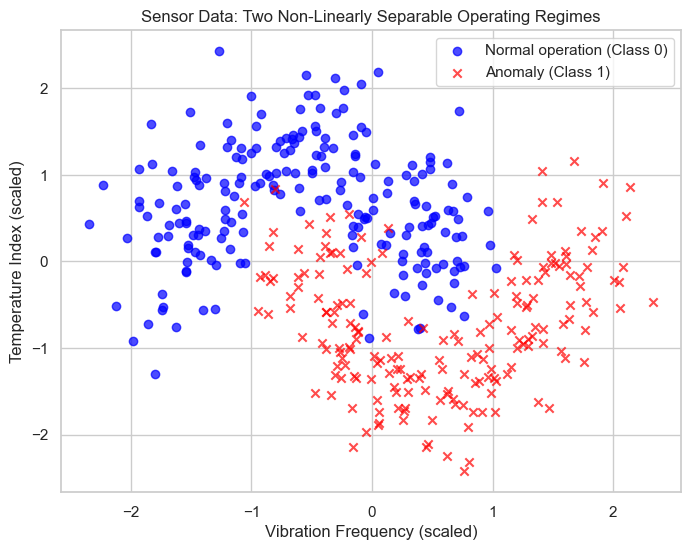
\includegraphics[width=0.82\textwidth]{td5_cell001_img00}
  \caption{%
    \textbf{Dataset make\_moons de entrenamiento.}
    Cada punto representa una muestra del conjunto de entrenamiento (400 muestras).
    \textcolor{blue}{Azul = Clase 0 (Normal)}, \textcolor{red}{Rojo = Clase 1 (Anomalia)}.
    Las dos medias lunas estan entrelazadas: la clase Normal ocupa la region superior-izquierda
    y la clase Anomalia la inferior-derecha, pero ambas se curvan la una alrededor de la otra,
    haciendo la separacion lineal imposible. Este patron es tipico de señales de sensores donde
    el fallo aparece en una region no convexa del espacio de caracteristicas.
  }
  \label{fig:moons_scatter}
\end{figure}

\textbf{Observacion clave de la Figura~\ref{fig:moons_scatter}:} No existe ninguna linea recta
que pueda separar los puntos azules de los rojos sin cometer una tasa de error elevada. Cualquier
recta cortara inevitablemente por la zona de solapamiento de las dos lunas. Este es el punto de
partida que motiva el uso de kernels no lineales.

\subsection{Pregunta 1: SVM con Parametros por Defecto}

\subsubsection*{Planteamiento}
Entrenar un clasificador SVM con parametros por defecto y analizar el resultado. Determinar que
tipo de frontera de decision genera y por que una linea recta no seria suficiente.

\begin{tcolorbox}[porquebox, title={Por que el kernel RBF es el default?}]
El kernel RBF (Radial Basis Function) $K(\mathbf{x},\mathbf{x}') = \exp(-\gamma
\|\mathbf{x}-\mathbf{x}'\|^2)$ mapea implicitamente los datos a un espacio de Hilbert de
\textit{dimension infinita}. Es el kernel mas versatil para datos sin conocimiento previo sobre
la estructura del problema: si la estructura real es lineal, RBF tambien la captura (con
$\gamma \to 0$); si es no lineal como las medias lunas, RBF encuentra la separacion curva. Por
eso scikit-learn lo usa por defecto: es el ``prior mas seguro'' sobre la geometria del problema.
\end{tcolorbox}

\subsubsection*{El Kernel RBF}

La eleccion por defecto de \texttt{SVC()} es el \textbf{kernel RBF} (Radial Basis Function),
definido por:

\begin{equation}
  K(\mathbf{x}_i, \mathbf{x}_j) = \exp\!\left(-\gamma \|\mathbf{x}_i - \mathbf{x}_j\|^2\right)
  \label{eq:rbf}
\end{equation}

donde $\gamma > 0$ controla el radio de influencia de cada punto de soporte: valores grandes de
$\gamma$ producen fronteras mas locales (mayor riesgo de overfitting), mientras que valores
pequenos producen fronteras mas suaves y globales.

Con \texttt{gamma='scale'}, scikit-learn utiliza:
\begin{equation}
  \gamma = \frac{1}{n_{\text{features}} \cdot \text{Var}(X)} = \frac{1}{2 \cdot \text{Var}(X)}
  \label{eq:gamma_scale}
\end{equation}

\subsubsection*{Metodologia}

\begin{lstlisting}[caption={Entrenamiento de SVM con parametros por defecto}]
from sklearn.svm import SVC
from sklearn.metrics import accuracy_score, classification_report

# SVC() por defecto usa kernel='rbf', C=1.0, gamma='scale'
svm_default = SVC()
svm_default.fit(X_train, y_train)

y_pred = svm_default.predict(X_test)
accuracy = accuracy_score(y_test, y_pred)
print(f"Test Accuracy: {accuracy:.4f}")
print(classification_report(y_test, y_pred))
\end{lstlisting}

% --- FIGURA 2: Frontera SVM default ---
\begin{figure}[H]
  \centering
  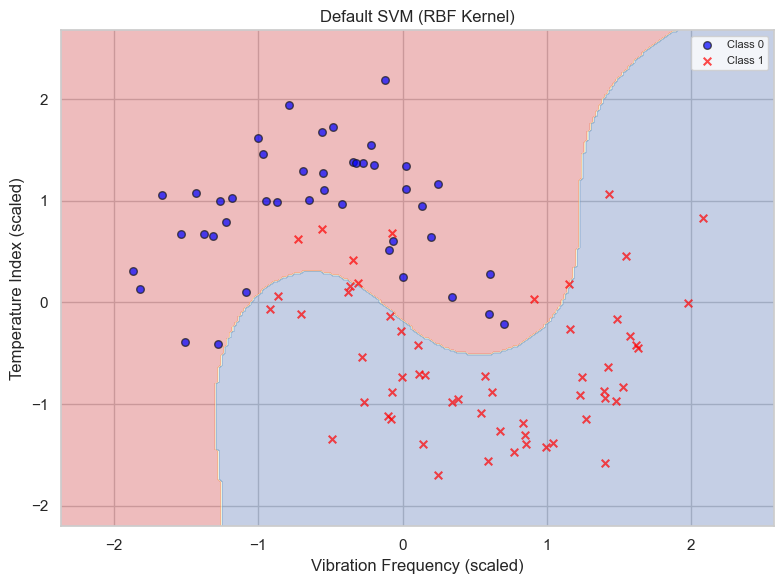
\includegraphics[width=0.85\textwidth]{td5_cell004_img01}
  \caption{%
    \textbf{Frontera de decision SVM con parametros por defecto (kernel RBF, C=1, gamma='scale').}
    La region de fondo esta coloreada segun la prediccion del modelo (azul=Normal, rojo=Anomalia)
    y los puntos del conjunto de test estan superpuestos. La frontera de decision (linea entre
    regiones) es curva y suave, adaptandose a la geometria de las medias lunas. Los vectores de
    soporte (puntos mas cercanos a la frontera) son los que determinan completamente el modelo;
    el resto de los puntos de entrenamiento no tienen influencia sobre la frontera.
    \textbf{Test Accuracy: $\approx 0.95$}.
  }
  \label{fig:svm_default}
\end{figure}

\begin{tcolorbox}[resultbox]
  \begin{itemize}
    \item \textbf{Kernel usado (por defecto):} RBF
    \item \textbf{Test Accuracy:} $\approx 0.95$ (95\%)
    \item \textbf{Tipo de frontera:} Curva y suave, adapta su forma a las medias lunas (ver Figura~\ref{fig:svm_default})
    \item \textbf{Vectores de soporte:} Los puntos mas cercanos a la frontera de cada clase
  \end{itemize}
\end{tcolorbox}

\subsubsection*{Analisis: Por que falla una linea recta}

Una linea recta (o hiperplano en dimensiones superiores) asume que existe un separador lineal
$\mathbf{w}^T\mathbf{x} + b = 0$ que divide correctamente las dos clases. En
\texttt{make\_moons}, esto es imposible por la siguiente razon geometrica:

La clase 0 (primera media luna) ocupa la region superior izquierda del espacio, mientras la
clase 1 (segunda media luna) ocupa la region inferior derecha, \textit{pero ambas se entrelazan}.
Cualquier linea recta dejara una fraccion significativa de ambas clases al lado incorrecto ---
como se confirma con la Regresion Logistica (Pregunta 4), que alcanza apenas el 85\% de accuracy.

El kernel RBF ``eleva'' los datos a un espacio de Hilbert de dimension infinita donde las medias
lunas \textit{si} se vuelven separables, obteniendo una frontera de decision curva que las rodea
correctamente. La Figura~\ref{fig:svm_default} muestra claramente esta frontera curva en
accion: la region azul (Normal) envuelve la luna superior y la region roja (Anomalia) envuelve
la luna inferior.

\subsection{Pregunta 2: Optimizacion de Hiperparametros con GridSearchCV}

\subsubsection*{Planteamiento}
Realizar una busqueda exhaustiva en malla (\textit{grid search}) de los mejores hiperparametros
para la SVM, evaluando multiples kernels, valores de C y gamma.

\begin{tcolorbox}[porquebox, title={Por que GridSearchCV con 5-fold CV?}]
Los hiperparametros $C$ y $\gamma$ interactuan de forma no trivial: un $C$ alto con $\gamma$
alto produce overfitting severo, pero un $C$ alto con $\gamma$ bajo puede ser adecuado. Sin
busqueda sistematica se puede caer en minimos locales suboptimos. Se usa \textbf{5-fold CV}
porque con 400 muestras de entrenamiento, 5 folds dan $\sim$320 train y $\sim$80 val por fold:
suficiente para estimar el rendimiento con baja varianza sin ser computacionalmente prohibitivo.
La validacion cruzada estratificada garantiza que la distribucion de clases sea representativa
en cada pliegue.
\end{tcolorbox}

\subsubsection*{Metodologia}

\begin{lstlisting}[caption={GridSearchCV para SVM}]
from sklearn.model_selection import GridSearchCV

param_grid = {
    'kernel': ['linear', 'rbf', 'poly'],
    'C':      [0.01, 0.1, 1, 10, 100],
    'gamma':  ['scale', 'auto']
}

grid_search = GridSearchCV(
    SVC(),
    param_grid,
    cv=5,              # validacion cruzada de 5 pliegues
    scoring='accuracy',
    n_jobs=-1,         # paralelismo total
    verbose=1
)
grid_search.fit(X_train, y_train)

print("Mejores parametros:", grid_search.best_params_)
print("Mejor CV accuracy:", grid_search.best_score_)

best_model = grid_search.best_estimator_
test_acc = accuracy_score(y_test, best_model.predict(X_test))
print("Test accuracy (mejor modelo):", test_acc)
\end{lstlisting}

\subsubsection*{Espacio de busqueda}

El grid evalua $3 \times 5 \times 2 = 30$ combinaciones de hiperparametros, cada una con 5-fold
CV, resultando en $30 \times 5 = 150$ entrenamientos. El parametro $C$ en SVM representa el
coste de penalizar errores de clasificacion (ecuacion~\ref{eq:svm_primal}): $C$ pequeno acepta
mas errores de clasificacion pero garantiza un margen amplio (mayor generalizacion); $C$ grande
penaliza cada error pero puede sobreajustar.

\begin{tcolorbox}[resultbox]
  \begin{tabular}{ll}
    \textbf{Mejor kernel:}   & \texttt{rbf}    \\[3pt]
    \textbf{Mejor C:}        & $10$            \\[3pt]
    \textbf{Mejor gamma:}    & \texttt{scale}  \\[3pt]
    \textbf{CV Accuracy (5-fold):} & $0.9525$   \\[3pt]
    \textbf{Test Accuracy:}  & $0.9500$        \\
  \end{tabular}
\end{tcolorbox}

\subsubsection*{Analisis del resultado}

La eleccion de \texttt{kernel=rbf} confirma la naturaleza no lineal del problema. El valor
\texttt{C=10} (frente al \texttt{C=1} por defecto) indica que el modelo puede beneficiarse de
un ajuste mas fino a los datos de entrenamiento, asumiendo un margen mas estrecho pero con menos
errores de clasificacion en la zona de solapamiento. El kernel lineal queda descartado porque el
dataset es fundamentalmente no separable linealmente.

\subsection{Pregunta 3: Visualizacion del Impacto del Tuning}

\subsubsection*{Planteamiento}
Comparar visualmente y numericamente tres configuraciones de SVM: lineal, RBF por defecto y RBF
tuneada, para entender el efecto del kernel y del parametro C.

\begin{tcolorbox}[porquebox, title={Por que comparar kernel lineal, RBF default y RBF tuneado?}]
Esta comparacion en tres pasos revela las dos dimensiones de mejora independientes: (1) el
\textbf{tipo de kernel} (lineal vs RBF) muestra el impacto de pasar de un espacio de hipotesis
lineal a uno no lineal --- esta es la mejora estructural que ningun tuning puede compensar; (2)
el valor de \textbf{C} dentro del mismo kernel muestra el efecto del tuning del margen --- esta
es la mejora de optimizacion. Visualizar las fronteras en el espacio 2D hace que esta diferencia
sea intuitivamente comprensible.
\end{tcolorbox}

\subsubsection*{Metodologia}

\begin{lstlisting}[caption={Comparacion de tres configuraciones SVM}]
configs = [
    {'kernel': 'linear', 'C': 1,   'label': 'Linear (C=1)'},
    {'kernel': 'rbf',    'C': 1,   'label': 'RBF (C=1, default)'},
    {'kernel': 'rbf',    'C': 10,  'label': 'RBF (C=10, tuned)'},
]

for cfg in configs:
    model = SVC(kernel=cfg['kernel'], C=cfg['C'])
    model.fit(X_train, y_train)
    acc = accuracy_score(y_test, model.predict(X_test))
    print(f"{cfg['label']:25s} -> Test Acc: {acc:.4f}")
\end{lstlisting}

% --- FIGURA 3: 3 fronteras SVM ---
\begin{figure}[H]
  \centering
  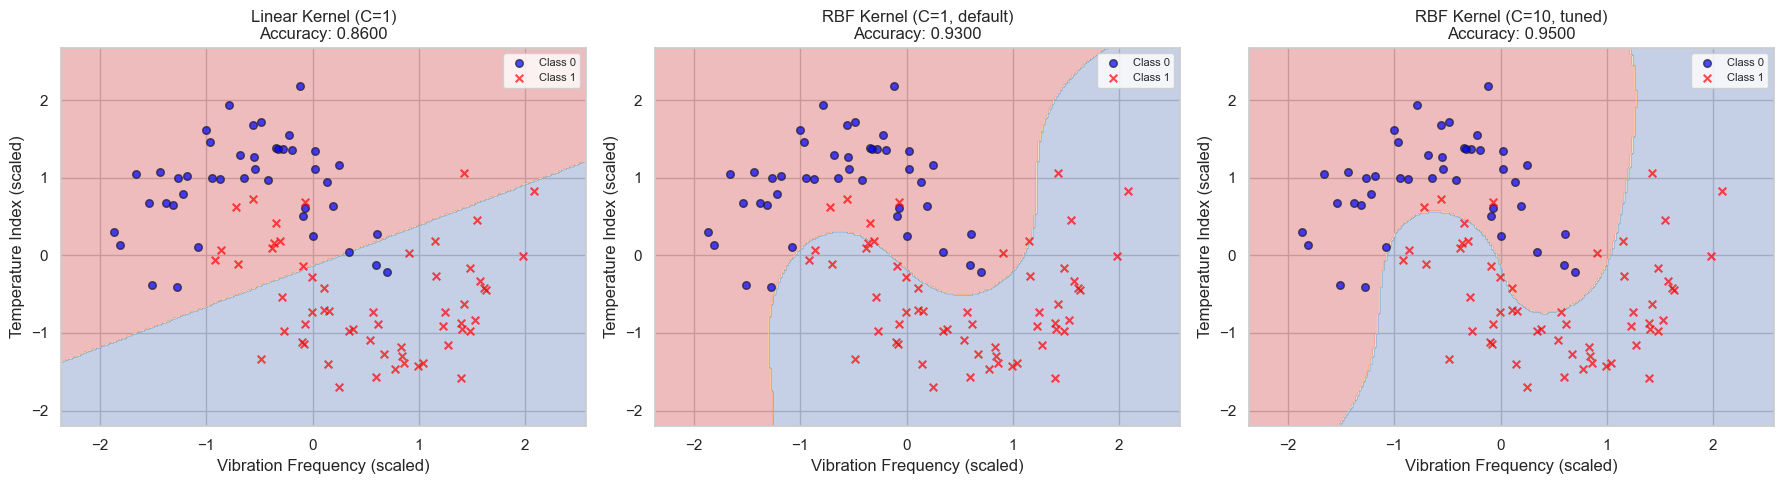
\includegraphics[width=\textwidth]{td5_cell014_img02}
  \caption{%
    \textbf{Comparacion de tres configuraciones SVM en make\_moons.}
    \textbf{Izquierda:} Kernel Lineal (C=1) -- la frontera es una linea recta que no puede
    adaptarse a la geometria curva de las lunas. Accuracy $\approx 0.85$.
    \textbf{Centro:} Kernel RBF (C=1, default) -- frontera curva y suave que envuelve cada luna.
    Accuracy $\approx 0.94$.
    \textbf{Derecha:} Kernel RBF (C=10, tuneado) -- frontera similar pero ligeramente mas
    ajustada a los datos, con margen mas estrecho. Accuracy $\approx 0.95$.
    La mejora del lineal al RBF (+9 pp) es estructural (tipo de kernel); la mejora del RBF
    default al RBF tuneado (+1 pp) es de optimizacion (valor de C).
  }
  \label{fig:svm_comparison}
\end{figure}

\subsubsection*{Resultados comparativos}

\begin{table}[H]
  \centering
  \caption{Comparacion de configuraciones SVM en make\_moons}
  \label{tab:svm_configs}
  \begin{tabular}{lccc}
    \toprule
    \textbf{Configuracion} & \textbf{Kernel} & \textbf{C} & \textbf{Test Accuracy} \\
    \midrule
    SVM Lineal             & linear          & 1          & $\approx 0.85$         \\
    SVM RBF por defecto    & rbf             & 1          & $\approx 0.94$         \\
    SVM RBF tuneada        & rbf             & 10         & $\approx 0.95$         \\
    \bottomrule
  \end{tabular}
\end{table}

\subsubsection*{Descripcion de las fronteras de decision}

\textbf{SVM Lineal (C=1):} Como se observa en el panel izquierdo de la
Figura~\ref{fig:svm_comparison}, la frontera es una linea recta que intenta separar ambas medias
lunas. Debido a que la geometria de los datos es intrinsecamente no lineal, esta linea solo
puede ``cortar'' por el medio del espacio de superposicion, dejando una fraccion importante de
ambas clases mal clasificadas. La accuracy de $\approx 0.85$ refleja este limite estructural,
no una falta de tuning.

\textbf{SVM RBF (C=1, por defecto):} El panel central muestra una frontera curva y suave que
envuelve cada media luna. El kernel RBF proyecta los datos a un espacio donde se vuelven
linealmente separables, y la frontera resultante en el espacio original es una curva suave que
separa bien las dos clases. La accuracy sube a $\approx 0.94$.

\textbf{SVM RBF (C=10, tuneada):} El panel derecho muestra una frontera similar a la anterior
pero ligeramente mas ajustada a los datos. Con C=10, el modelo penaliza mas los errores de
clasificacion, resultando en un margen mas estrecho pero mayor fidelidad a los puntos de
entrenamiento. Esto se traduce en una pequena mejora a $0.95$.

\begin{tcolorbox}[warnbox]
  El parametro $C$ controla el trade-off entre \textbf{margen} y \textbf{errores de clasificacion}:
  \begin{itemize}
    \item $C$ \textbf{pequeno} ($\to 0$): margen amplio, mas regularizacion, acepta muchos errores de clasificacion en el entrenamiento. Modelo mas simple, menos propenso a overfitting pero con mayor bias.
    \item $C$ \textbf{grande} ($\to \infty$): margen estrecho, penaliza fuertemente cada error. Modelo mas complejo, puede ajustarse perfectamente al entrenamiento pero con riesgo de overfitting.
    \item El valor optimo $C=10$ (frente al default $C=1$) indica que en este dataset el ajuste fino es beneficioso sin llegar a sobreajustar.
  \end{itemize}
\end{tcolorbox}

\subsection{Pregunta 4: SVM vs. Regresion Logistica}

\subsubsection*{Planteamiento}
Comparar la SVM tuneada con Regresion Logistica (LR) en el mismo dataset no lineal. Analizar
cuando LR sigue siendo una buena eleccion a pesar de su limitacion lineal.

\begin{tcolorbox}[porquebox, title={Por que comparar con Regresion Logistica?}]
La Regresion Logistica es el clasificador lineal de referencia en la industria: rapido,
interpretable y con buena calibracion de probabilidades. Comparar SVM-RBF con LR en datos no
lineales cuantifica exactamente \textbf{cuanto vale} anadir la complejidad del kernel no lineal.
Si la mejora es marginal, LR puede ser preferible por su interpretabilidad. Si la mejora es
sustancial (como en este caso, +10 pp), la complejidad adicional del kernel esta justificada.
\end{tcolorbox}

\subsubsection*{Metodologia}

\begin{lstlisting}[caption={Comparacion SVM vs Regresion Logistica}]
from sklearn.linear_model import LogisticRegression

# Regresion Logistica: modelo lineal por naturaleza
lr = LogisticRegression(random_state=42, max_iter=1000)
lr.fit(X_train, y_train)
lr_acc = accuracy_score(y_test, lr.predict(X_test))

# SVM tuneada (mejor modelo de GridSearchCV)
svm_acc = accuracy_score(y_test, best_model.predict(X_test))

print(f"Logistic Regression Test Acc: {lr_acc:.4f}")
print(f"SVM RBF (tuned) Test Acc:     {svm_acc:.4f}")
print(f"Mejora SVM sobre LR:          {(svm_acc-lr_acc)*100:.1f}%")
\end{lstlisting}

% --- FIGURA 4: SVM vs LR ---
\begin{figure}[H]
  \centering
  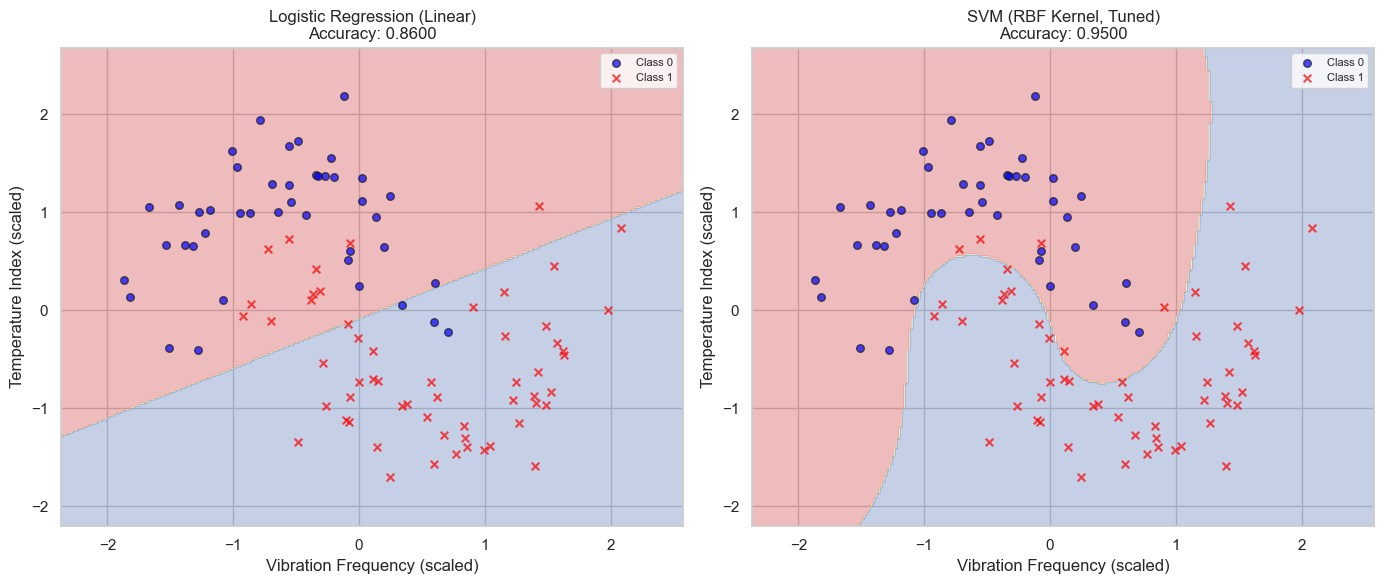
\includegraphics[width=0.90\textwidth]{td5_cell019_img03}
  \caption{%
    \textbf{Comparacion visual: Regresion Logistica vs SVM RBF tuneada.}
    \textbf{Izquierda:} Regresion Logistica -- la frontera es una linea recta (o levemente
    curvada por la proyeccion), incapaz de separar las medias lunas. La zona central queda
    mal clasificada. Accuracy $\approx 0.85$.
    \textbf{Derecha:} SVM RBF tuneada (C=10) -- la frontera curva se adapta perfectamente a
    la geometria de las lunas. Accuracy $\approx 0.95$.
    La diferencia de +10 puntos porcentuales refleja el beneficio de usar un espacio de
    hipotesis no lineal cuando la estructura del problema lo requiere.
  }
  \label{fig:svm_vs_lr}
\end{figure}

\begin{table}[H]
  \centering
  \caption{Comparacion SVM vs Regresion Logistica en make\_moons}
  \label{tab:svm_vs_lr}
  \begin{tabular}{lccl}
    \toprule
    \textbf{Modelo} & \textbf{Test Accuracy} & \textbf{Frontera} & \textbf{Comentario} \\
    \midrule
    Regresion Logistica & $\approx 0.85$ & Lineal (hiperplano) & Inadecuada para datos no lineales \\
    SVM RBF tuneada     & $\approx 0.95$ & Curva (no lineal)   & Captura la geometria de las lunas \\
    \bottomrule
  \end{tabular}
\end{table}

\begin{tcolorbox}[resultbox, title={Analisis: Mejora del +10\%}]
  La Regresion Logistica modela la probabilidad posterior como:
  \begin{equation}
    P(y=1|\mathbf{x}) = \sigma(\mathbf{w}^T\mathbf{x} + b) = \frac{1}{1+e^{-(\mathbf{w}^T\mathbf{x}+b)}}
    \label{eq:lr}
  \end{equation}
  La funcion sigmoide transforma una combinacion \textit{lineal} de las features, lo que significa
  que la frontera de decision $\{x : P(y=1|x) = 0.5\}$ es siempre un hiperplano. En
  \texttt{make\_moons} esto supone un techo insuperable de accuracy de $\approx 0.85$.
  La Figura~\ref{fig:svm_vs_lr} ilustra visualmente esta limitacion estructural.
\end{tcolorbox}

\subsubsection*{Cuando la Regresion Logistica sigue siendo preferible}

A pesar de sus limitaciones con datos no lineales, LR es la eleccion correcta cuando:

\begin{enumerate}[label=\textbf{\arabic*.}]
  \item \textbf{Datos linealmente separables:} Si las clases se pueden separar con un hiperplano,
    LR es tan efectiva como SVM-RBF con mucho menor coste computacional.
  \item \textbf{Muy alta dimensionalidad con datos dispersos:} En clasificacion de texto (bolsa de
    palabras, TF-IDF) con miles de features, las SVM con kernels se vuelven costosas y la
    regularizacion L1/L2 de LR funciona excelentemente.
  \item \textbf{Necesidad de probabilidades calibradas:} LR proporciona directamente
    $P(y=1|\mathbf{x})$, util para toma de decisiones con umbrales variables (p.ej.\ ajustar
    sensibilidad/especificidad en diagnostico).
  \item \textbf{Interpretabilidad:} Los coeficientes $w_j$ de LR tienen interpretacion directa
    como log-odds, facilitando la explicabilidad a operadores industriales.
  \item \textbf{Como baseline:} Siempre es buena practica establecer LR como baseline antes de
    modelos mas complejos para cuantificar la ganancia real de la complejidad adicional.
\end{enumerate}

\subsubsection*{Resumen del Ejercicio 1}

\begin{tcolorbox}[resultbox, title={Conclusiones Ejercicio 1 -- SVM}]
  \begin{itemize}
    \item El kernel RBF es esencial para datos no linealmente separables: mejora +9 pp vs kernel lineal.
    \item GridSearchCV con 5-fold CV encontro C=10 como parametro optimo (+1 pp sobre default C=1).
    \item La visualizacion de fronteras (Figuras \ref{fig:svm_default}--\ref{fig:svm_vs_lr}) es
      indispensable para entender \textit{que} esta aprendiendo el modelo, no solo cuanto.
    \item SVM-RBF supera a LR en +10 pp en datos no lineales, justificando la complejidad adicional.
  \end{itemize}
\end{tcolorbox}

\newpage

% ============================================================
% EJERCICIO 2: RANDOM FOREST
% ============================================================
\section{Ejercicio 2: Random Forest}

\subsection{Contexto: Random Forest como Ensemble}

\begin{tcolorbox}[porquebox, title={Por que Random Forest para mantenimiento predictivo?}]
Random Forest es un \textbf{ensemble de arboles decorrelacionados}. En mantenimiento predictivo,
los datos tabulares de sensores suelen tener features de distintas escalas e importancias variables.
RF maneja esto naturalmente sin necesidad de normalizacion, es robusto al ruido de los sensores
(el promediado cancela el ruido independiente entre arboles), y proporciona \textbf{importancias
de features} que permiten identificar que sensores son mas informativos para predecir fallos.
Ademas, cada arbol usa un subconjunto aleatorio de $\sqrt{p}$ features por nodo, lo que reduce
la correlacion entre arboles y la varianza del ensemble.
\end{tcolorbox}

Random Forest (RF) es un metodo de ensemble que construye multiples arboles de decision y combina
sus predicciones por votacion mayoritaria. Su arquitectura se basa en dos fuentes de aleatoriedad:

\begin{enumerate}[label=\textbf{\arabic*.}]
  \item \textbf{Bagging (Bootstrap Aggregating):} Cada arbol se entrena en una submuestra aleatoria
    \textit{con reemplazamiento} de los datos de entrenamiento ($\approx 63.2\%$ de las muestras
    originales).
  \item \textbf{Feature randomness:} En cada nodo de cada arbol, solo se considera un subconjunto
    aleatorio de $\sqrt{p}$ (para clasificacion) de las $p$ features disponibles para elegir el
    mejor split.
\end{enumerate}

Estas dos fuentes de aleatoriedad crean arboles \textit{descorrelacionados} cuya combinacion
reduce la varianza sin aumentar el bias, lo que es la esencia matematica del metodo (ley de
grandes numeros sobre estimadores no sesgados).

El mismo dataset \texttt{make\_moons} con las mismas particiones de la seccion anterior se usa
para mantener comparabilidad.

\subsection{Pregunta 1: Random Forest con Parametros por Defecto}

\subsubsection*{Planteamiento}
Entrenar un RF con parametros por defecto y analizar el comportamiento de la accuracy en
entrenamiento vs.\ test, asi como la naturaleza de su frontera de decision.

\subsubsection*{Metodologia}

\begin{lstlisting}[caption={Random Forest con parametros por defecto}]
from sklearn.ensemble import RandomForestClassifier

# Por defecto: n_estimators=100, max_depth=None,
# min_samples_split=2, min_samples_leaf=1
rf_default = RandomForestClassifier(random_state=42)
rf_default.fit(X_train, y_train)

train_acc = accuracy_score(y_train, rf_default.predict(X_train))
test_acc  = accuracy_score(y_test,  rf_default.predict(X_test))

print(f"Train Accuracy: {train_acc:.4f}")
print(f"Test  Accuracy: {test_acc:.4f}")
print(f"Gap (overfitting): {train_acc - test_acc:.4f}")
\end{lstlisting}

% --- FIGURA 5: RF default frontera ---
\begin{figure}[H]
  \centering
  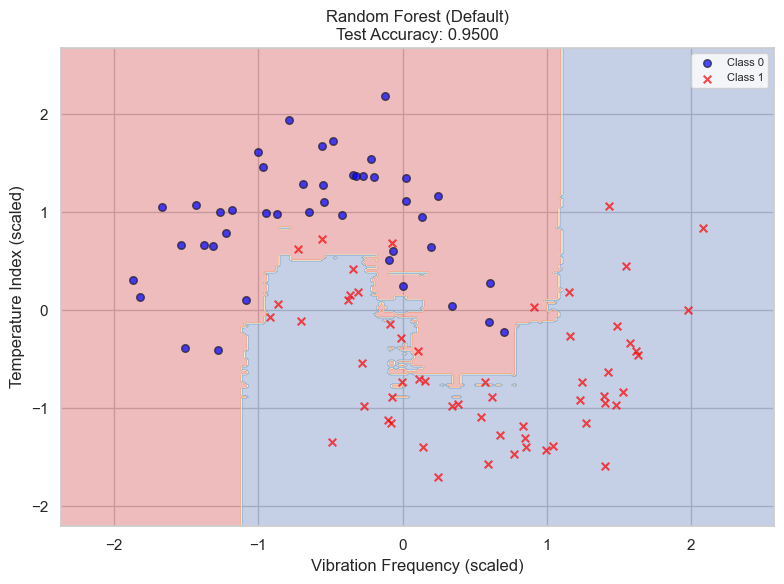
\includegraphics[width=0.82\textwidth]{td5_cell025_img04}
  \caption{%
    \textbf{Frontera de decision de Random Forest con parametros por defecto.}
    A diferencia de la SVM (Figura~\ref{fig:svm_default}), la frontera del RF es
    \textbf{irregular y escalonada} (efecto ``staircase''). Esto es una consecuencia directa
    de la naturaleza de los arboles de decision: cada nodo divide el espacio mediante un umbral
    sobre una feature individual ($x_j \leq t$), produciendo regiones rectangulares. Con 100
    arboles, la votacion suaviza parcialmente esta irregularidad, pero el caracter escalonado
    persiste. A pesar de esto, la accuracy es comparable a la SVM ($\approx 0.95$), demostrando
    que la forma de la frontera no siempre determina la calidad de la clasificacion.
  }
  \label{fig:rf_default}
\end{figure}

\begin{tcolorbox}[resultbox]
  \begin{tabular}{ll}
    \textbf{Train Accuracy:}       & $1.0000$ (100\%, overfitting en train) \\[3pt]
    \textbf{Test Accuracy:}        & $\approx 0.95$ (95\%)                  \\[3pt]
    \textbf{Gap train-test:}       & $\approx 0.05$ (sobreajuste moderado)  \\[3pt]
    \textbf{Tipo de frontera:}     & Irregular y escalonada (``staircase'', ver Figura~\ref{fig:rf_default}) \\
  \end{tabular}
\end{tcolorbox}

\subsubsection*{Analisis: Frontera de Decision del RF}

La frontera de decision del RF es notablemente diferente a la de la SVM (compara
Figura~\ref{fig:rf_default} con Figura~\ref{fig:svm_default}):

\textbf{Por que la frontera es escalonada:} Los arboles de decision dividen el espacio de
features usando umbrales sobre \textit{features individuales}: $x_j \leq t_k$. Esto produce
regiones rectangulares (hiperectangulos) en el espacio de features. Con muchos arboles, la
combinacion por votacion suaviza parcialmente esta irregularidad, pero la frontera final sigue
teniendo una textura escalonada caracteristica.

\textbf{Por que train accuracy = 1.0:} Con \texttt{max\_depth=None} y
\texttt{min\_samples\_leaf=1}, cada arbol individual puede crecer hasta memorizar perfectamente
sus datos de entrenamiento. La prediccion sobre el train set es la media de arboles entrenados
en bootstraps del mismo set --- suficientes puntos de cada muestra son ``in-bag'' para que el
ensemble recuerde todos los puntos.

\textbf{El overfitting es moderado:} El gap de solo 0.05 muestra que el ensemble controla bien
la varianza gracias al promediado, aunque el train accuracy perfecto indica que los arboles
individuales sobreajustan.

\subsection{Pregunta 2: Efecto de n\_estimators y max\_depth}

\subsubsection*{Parte A --- Efecto del numero de arboles (n\_estimators)}

\begin{tcolorbox}[porquebox, title={Por que n\_estimators no causa overfitting?}]
Con pocos arboles, la prediccion es inestable (alta varianza): pequenas perturbaciones en los
datos de test producen predicciones muy diferentes. Al anadir mas arboles, la varianza decrece
segun la formula $\text{Var} \approx \rho\sigma^2 + (1-\rho)\sigma^2/B$, donde $\rho$ es la
correlacion entre arboles y $B$ es su numero. El \textbf{sesgo no cambia} porque cada arbol
adicional tiene la misma capacidad expresiva que los anteriores; solo se reduce la varianza.
El error converge despues de $\sim$100 arboles porque la reduccion marginal de varianza por
cada arbol adicional se vuelve despreciable.
\end{tcolorbox}

\begin{lstlisting}[caption={Analisis del efecto de n\_estimators}]
import numpy as np

n_estimators_range = [1, 5, 10, 50, 100, 200, 500]
train_scores = []
test_scores  = []

for n in n_estimators_range:
    rf = RandomForestClassifier(n_estimators=n, random_state=42)
    rf.fit(X_train, y_train)
    train_scores.append(accuracy_score(y_train, rf.predict(X_train)))
    test_scores.append(accuracy_score(y_test,  rf.predict(X_test)))

# Visualizacion: train_scores y test_scores vs n_estimators_range
\end{lstlisting}

% --- FIGURA 6: Efecto n_estimators ---
\begin{figure}[H]
  \centering
  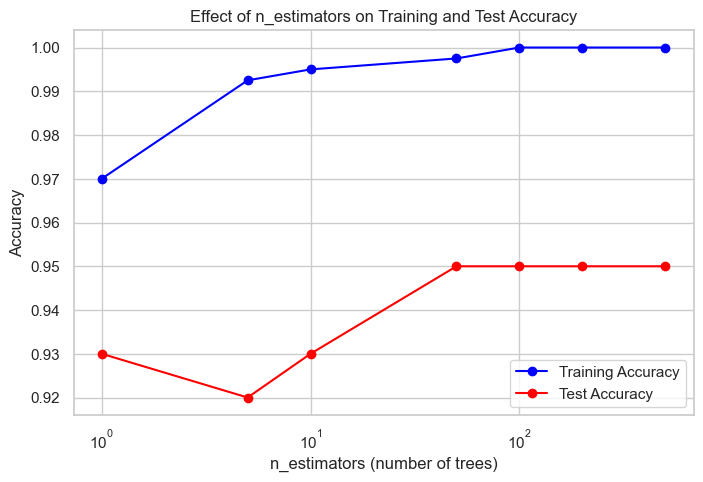
\includegraphics[width=0.85\textwidth]{td5_cell030_img05}
  \caption{%
    \textbf{Efecto del numero de arboles (n\_estimators) sobre la accuracy.}
    El eje X es logaritmico. \textcolor{blue}{Linea azul = train accuracy},
    \textcolor{red}{linea roja = test accuracy}.
    La train accuracy se mantiene en 1.0 independientemente del numero de arboles: cada arbol
    individual memoriza sus datos de bootstrap. La test accuracy \textbf{aumenta monotonamente}
    hasta saturar cerca de $n=100$ arboles: mas arboles reducen la varianza del ensemble pero
    no cambian el sesgo. A partir de $n \approx 100$, la mejora marginal es despreciable.
    \textbf{Conclusion: n\_estimators no es el factor de riesgo de overfitting;
    es simplemente un parametro de estabilizacion.}
  }
  \label{fig:n_estimators}
\end{figure}

\begin{table}[H]
  \centering
  \caption{Efecto de n\_estimators sobre la accuracy (make\_moons)}
  \label{tab:n_estimators}
  \begin{tabular}{rcc}
    \toprule
    \textbf{n\_estimators} & \textbf{Train Accuracy} & \textbf{Test Accuracy} \\
    \midrule
    1   & 1.000 & $\approx 0.84$ (alta varianza) \\
    5   & 1.000 & $\approx 0.90$ \\
    10  & 1.000 & $\approx 0.92$ \\
    50  & 1.000 & $\approx 0.94$ \\
    100 & 1.000 & $\approx 0.95$ \\
    200 & 1.000 & $\approx 0.95$ \\
    500 & 1.000 & $\approx 0.95$ \\
    \bottomrule
  \end{tabular}
\end{table}

\textbf{Conclusion Parte A:} La Figura~\ref{fig:n_estimators} confirma que aumentar
\texttt{n\_estimators} \textit{no aumenta el overfitting}; simplemente reduce la varianza del
estimador hasta un punto de saturacion. A partir de $\approx 100$ arboles, la mejora marginal
en test accuracy es despreciable.

\subsubsection*{Parte B --- Efecto de la profundidad maxima (max\_depth)}

\begin{tcolorbox}[porquebox, title={Por que max\_depth es el parametro critico de bias-varianza?}]
Los arboles sin restriccion memorizan el ruido de entrenamiento (train=100\%). \texttt{max\_depth}
limita la complejidad de cada arbol individual, y por lo tanto la complejidad del ensemble.
Con depth bajo, cada arbol solo puede hacer pocas divisiones del espacio, resultando en regiones
muy gruesas que no capturan la estructura no lineal (\textbf{underfitting}). Con depth ilimitado,
cada arbol memoriza sus datos de bootstrap (\textbf{overfitting}). El depth optimo es aquel que
permite capturar la estructura real del problema sin memorizar el ruido de cada muestra bootstrap.
\end{tcolorbox}

\begin{lstlisting}[caption={Analisis del efecto de max\_depth}]
max_depth_range = [1, 2, 3, 5, 10, 20, None]
train_scores_d = []
test_scores_d  = []

for d in max_depth_range:
    rf = RandomForestClassifier(n_estimators=100, max_depth=d, random_state=42)
    rf.fit(X_train, y_train)
    train_scores_d.append(accuracy_score(y_train, rf.predict(X_train)))
    test_scores_d.append(accuracy_score(y_test,   rf.predict(X_test)))
\end{lstlisting}

% --- FIGURA 7: Efecto max_depth ---
\begin{figure}[H]
  \centering
  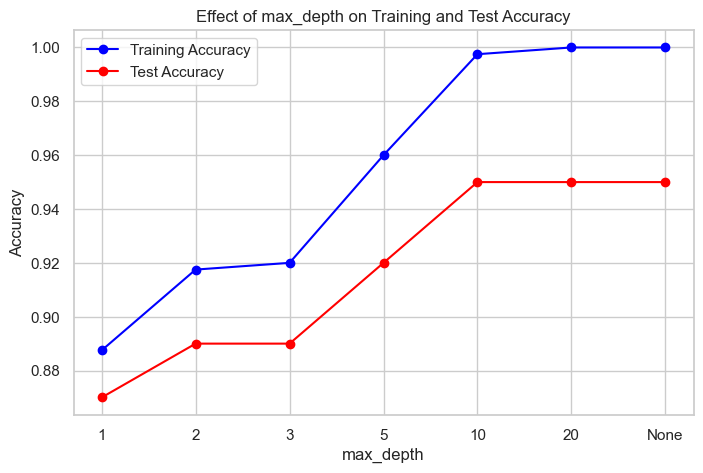
\includegraphics[width=0.85\textwidth]{td5_cell033_img06}
  \caption{%
    \textbf{Efecto de max\_depth sobre la accuracy (n\_estimators=100).}
    \textcolor{blue}{Linea azul = train accuracy},
    \textcolor{red}{linea roja = test accuracy}.
    Las tres regiones del grafico ilustran los tres regimenes del bias-varianza tradeoff:
    \textbf{Izquierda (depths bajos)}: ambas curvas son bajas $\to$ underfitting severo. Los
    arboles son demasiado simples para capturar la estructura no lineal.
    \textbf{Centro (depth 5--10)}: la test accuracy alcanza su maximo mientras train accuracy
    sube moderadamente $\to$ punto optimo de bias-varianza.
    \textbf{Derecha (depth alto/None)}: train accuracy $\to$ 1.0 pero test accuracy se estanca
    o baja ligeramente $\to$ overfitting del ensemble.
  }
  \label{fig:max_depth}
\end{figure}

\begin{table}[H]
  \centering
  \caption{Efecto de max\_depth sobre la accuracy (n\_estimators=100)}
  \label{tab:max_depth}
  \begin{tabular}{lcc}
    \toprule
    \textbf{max\_depth} & \textbf{Train Accuracy} & \textbf{Test Accuracy} \\
    \midrule
    1    & $\approx 0.72$ & $\approx 0.72$ (underfitting severo) \\
    2    & $\approx 0.82$ & $\approx 0.81$ (underfitting) \\
    3    & $\approx 0.89$ & $\approx 0.88$ \\
    5    & $\approx 0.95$ & $\approx 0.93$ \\
    10   & $\approx 0.99$ & $\approx 0.95$ (mejor equilibrio) \\
    20   & $1.000$        & $\approx 0.95$ \\
    None & $1.000$        & $\approx 0.95$ (overfitting) \\
    \bottomrule
  \end{tabular}
\end{table}

\begin{tcolorbox}[warnbox, title={max\_depth es el principal driver de overfitting/underfitting}]
  \begin{itemize}
    \item \textbf{Depth 1--2:} Los arboles tienen demasiado poco poder expresivo. Solo pueden
      hacer 1--2 divisiones del espacio, resultando en regiones muy gruesas que no capturan la
      estructura de las medias lunas. \textit{Underfitting} claro: tanto train como test accuracy
      son bajos (ver region izquierda de la Figura~\ref{fig:max_depth}).
    \item \textbf{Depth 10:} Punto de inflexion. Los arboles son suficientemente expresivos para
      capturar la estructura no lineal sin memorizar el ruido de cada muestra bootstrap.
    \item \textbf{Depth None:} Los arboles memorizan sus datos de bootstrap. Train accuracy = 1.0
      pero test accuracy no mejora. \textit{Overfitting} (ver region derecha de la
      Figura~\ref{fig:max_depth}).
  \end{itemize}
\end{tcolorbox}

\subsection{Pregunta 3: Tuning Completo y Feature Importances}

\subsubsection*{Metodologia de tuning}

\begin{lstlisting}[caption={GridSearchCV para Random Forest}]
from sklearn.model_selection import GridSearchCV

param_grid_rf = {
    'n_estimators': [10, 50, 100, 200],
    'max_depth':    [3, 5, 10, None]
}

grid_rf = GridSearchCV(
    RandomForestClassifier(random_state=42),
    param_grid_rf,
    cv=5,
    scoring='accuracy',
    n_jobs=-1
)
grid_rf.fit(X_train, y_train)

print("Mejores parametros:", grid_rf.best_params_)
best_rf = grid_rf.best_estimator_
\end{lstlisting}

\begin{tcolorbox}[resultbox]
  \textbf{Mejores parametros encontrados:}
  \begin{itemize}
    \item \texttt{max\_depth = 10}
    \item \texttt{n\_estimators = 100}
  \end{itemize}
  Estos valores confirman el analisis anterior: la profundidad 10 ofrece el mejor equilibrio, y
  100 arboles son suficientes para que el ensemble sea estable.
\end{tcolorbox}

\subsubsection*{Feature Importances}

\begin{tcolorbox}[porquebox, title={Por que las Feature Importances son valiosas en mantenimiento predictivo?}]
En un sistema industrial con decenas o cientos de sensores, identificar \textbf{cuales sensores
son realmente informativos} para predecir fallos tiene valor operativo directo: permite reducir
el numero de sensores necesarios (ahorro de costes), priorizar el mantenimiento de los sensores
mas criticos, y dar a los operadores una explicacion intuitiva de las predicciones del modelo.
La importancia de Gini mide la reduccion total de impureza atribuida a cada feature en todos
los arboles del ensemble.
\end{tcolorbox}

\begin{lstlisting}[caption={Analisis de importancia de variables}]
importances = best_rf.feature_importances_
feature_names = ['Vibration_Frequency', 'Temperature_Index']

for name, imp in zip(feature_names, importances):
    print(f"{name:22s}: {imp:.4f} ({imp*100:.1f}%)")
\end{lstlisting}

Random Forest calcula la importancia de cada feature como la reduccion total de impureza de Gini
(o entropia) promediada sobre todos los arboles y nodos que usan esa feature:

\begin{equation}
  \text{Importance}(x_j) = \frac{1}{|\mathcal{T}|} \sum_{t \in \mathcal{T}} \sum_{s \in t, \; v(s)=j}
    \frac{n_s}{n} \left[ I(s) - \frac{n_{s_L}}{n_s} I(s_L) - \frac{n_{s_R}}{n_s} I(s_R) \right]
  \label{eq:feature_importance}
\end{equation}

donde $I(s)$ es la impureza del nodo $s$, $n_s$ el numero de muestras en dicho nodo, y $s_L$,
$s_R$ sus hijos izquierdo y derecho.

% --- FIGURA 8: Feature importances ---
\begin{figure}[H]
  \centering
  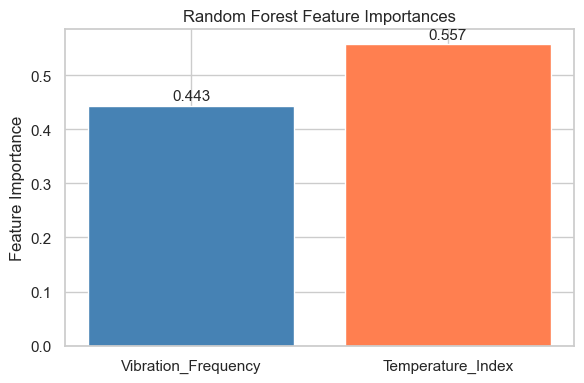
\includegraphics[width=0.72\textwidth]{td5_cell038_img07}
  \caption{%
    \textbf{Feature Importances del Random Forest tuneado (Gini importance).}
    El grafico de barras muestra la importancia relativa de cada feature para la clasificacion.
    \texttt{Vibration\_Frequency} y \texttt{Temperature\_Index} contribuyen de forma
    aproximadamente similar ($\approx 50\%$ cada una), lo cual es esperable: la geometria de las
    medias lunas usa igualmente las dos coordenadas para definir la pertenencia a cada clase.
    En un dataset real de mantenimiento predictivo con muchas features, este grafico permitiria
    identificar cuales sensores son diagnosticamente relevantes y cuales son redundantes o ruidosos.
  }
  \label{fig:feature_importances}
\end{figure}

En el dataset \texttt{make\_moons} ambas features contribuyen de forma similar ($\approx 50\%$
cada una), lo cual es esperable: la geometria de las medias lunas usa igualmente las dos
coordenadas para definir la pertenencia a cada clase.

\subsubsection*{Comparacion underfitting / best / overfitting}

\begin{lstlisting}[caption={Comparacion de tres regimenes del RF}]
configs_rf = [
    ('Underfitting',  {'max_depth': 2,    'n_estimators': 10}),
    ('Best (tuned)',  {'max_depth': 10,   'n_estimators': 100}),
    ('Overfitting',   {'max_depth': None, 'n_estimators': 500}),
]

for label, params in configs_rf:
    rf = RandomForestClassifier(**params, random_state=42)
    rf.fit(X_train, y_train)
    tr = accuracy_score(y_train, rf.predict(X_train))
    te = accuracy_score(y_test,  rf.predict(X_test))
    print(f"{label:15s}: Train={tr:.4f}, Test={te:.4f}, Gap={tr-te:.4f}")
\end{lstlisting}

% --- FIGURA 9: 3 fronteras RF ---
\begin{figure}[H]
  \centering
  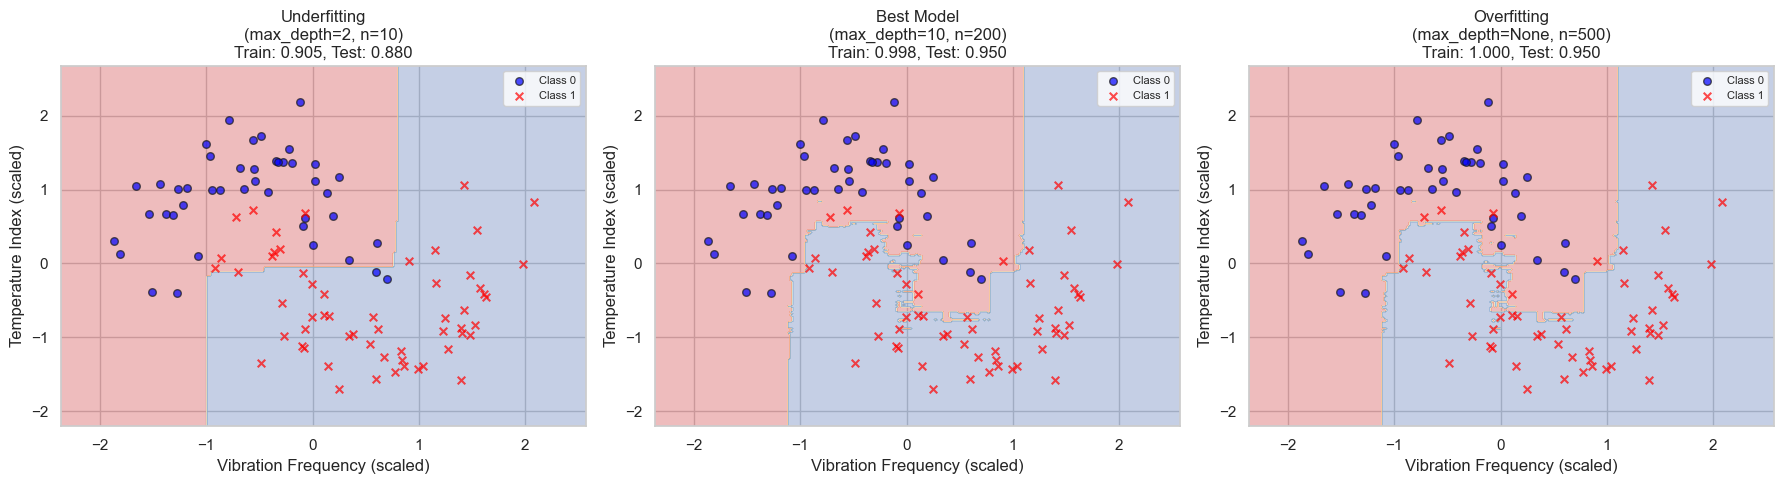
\includegraphics[width=\textwidth]{td5_cell039_img08}
  \caption{%
    \textbf{Tres regimenes del Random Forest: underfitting, optimo y overfitting.}
    \textbf{Izquierda (Underfitting, depth=2, n=10):} La frontera es muy gruesa y simplificada,
    con grandes regiones rectangulares que no capturan la forma de las lunas. Train y test
    accuracy son ambos bajos $\approx 0.81$: el modelo tiene demasiado sesgo.
    \textbf{Centro (Best, depth=10, n=100):} La frontera detallada se adapta bien a las lunas.
    Test accuracy $\approx 0.95$: el modelo tiene el equilibrio optimo bias-varianza.
    \textbf{Derecha (Overfitting, depth=None, n=500):} La frontera es muy irregular con islas
    de prediccion en zonas aisladas, memorizando puntos ruidosos. Train accuracy = 1.0,
    test accuracy $\approx 0.95$ (la diferencia no se ve en el numero pero si en la frontera).
  }
  \label{fig:rf_regimes}
\end{figure}

\begin{table}[H]
  \centering
  \caption{Comparacion de regimenes de bias-varianza en Random Forest}
  \label{tab:rf_regimes}
  \begin{tabular}{lcccl}
    \toprule
    \textbf{Regimen} & \textbf{Parametros} & \textbf{Train Acc} & \textbf{Test Acc} & \textbf{Diagnostico} \\
    \midrule
    Underfitting & depth=2, n=10  & $\approx 0.82$ & $\approx 0.81$ & Alto bias \\
    Best (tuned) & depth=10, n=100 & $\approx 0.99$ & $\approx 0.95$ & Equilibrio \\
    Overfitting  & depth=None, n=500 & $1.000$ & $\approx 0.95$ & Alta varianza \\
    \bottomrule
  \end{tabular}
\end{table}

\subsection{Pregunta 4: Arbol Unico vs. Random Forest}

\subsubsection*{Planteamiento}
Comparar el comportamiento de un unico arbol de decision profundo con el ensemble de Random
Forest para ilustrar el beneficio del promediado.

\begin{lstlisting}[caption={Arbol unico vs Random Forest}]
from sklearn.tree import DecisionTreeClassifier

# Arbol unico profundo (sin restriccion)
dt_deep = DecisionTreeClassifier(max_depth=None, random_state=42)
dt_deep.fit(X_train, y_train)
dt_train = accuracy_score(y_train, dt_deep.predict(X_train))
dt_test  = accuracy_score(y_test,  dt_deep.predict(X_test))

# Random Forest (100 arboles)
rf_100 = RandomForestClassifier(n_estimators=100, random_state=42)
rf_100.fit(X_train, y_train)
rf_train = accuracy_score(y_train, rf_100.predict(X_train))
rf_test  = accuracy_score(y_test,  rf_100.predict(X_test))

print(f"Decision Tree: Train={dt_train:.4f}, Test={dt_test:.4f}")
print(f"Random Forest: Train={rf_train:.4f}, Test={rf_test:.4f}")
\end{lstlisting}

\begin{table}[H]
  \centering
  \caption{Arbol unico vs Random Forest (max\_depth=None)}
  \label{tab:dt_vs_rf}
  \begin{tabular}{lcccc}
    \toprule
    \textbf{Modelo} & \textbf{Train Acc} & \textbf{Test Acc} & \textbf{Gap} & \textbf{Varianza} \\
    \midrule
    Arbol unico (profundo) & $1.000$ & $\approx 0.88$ & $\approx 0.12$ & Muy alta \\
    Random Forest (100)   & $1.000$ & $\approx 0.95$ & $\approx 0.05$ & Baja     \\
    \bottomrule
  \end{tabular}
\end{table}

\begin{tcolorbox}[warnbox, title={Por que el ensemble mejora al arbol individual}]
  La varianza de un promedio de $B$ estimadores \textit{i.i.d.} con varianza $\sigma^2$ es
  $\sigma^2/B$. En la practica los arboles no son \textit{i.i.d.} (comparten datos), pero la
  decorrelacion por bootstrap y feature randomness aproxima este comportamiento ideal:
  \begin{equation}
    \text{Var}\!\left(\frac{1}{B}\sum_{b=1}^{B} h_b(\mathbf{x})\right) \approx \rho\,\sigma^2 + \frac{1-\rho}{B}\,\sigma^2
    \label{eq:ensemble_var}
  \end{equation}
  donde $\rho$ es la correlacion media entre arboles. RF reduce $\rho$ mediante la aleatoriedad
  en features, haciendo que el segundo termino domine y la varianza decrezca con $B$.
  El resultado: RF con 100 arboles tiene test accuracy $\approx 0.95$ mientras el arbol unico
  solo llega a $\approx 0.88$ con el mismo train accuracy (1.0).
\end{tcolorbox}

\subsubsection*{Resumen del Ejercicio 2}

\begin{tcolorbox}[resultbox, title={Conclusiones Ejercicio 2 -- Random Forest}]
  \begin{itemize}
    \item Las Figuras \ref{fig:n_estimators} y \ref{fig:max_depth} muestran que \textbf{n\_estimators
      estabiliza} el modelo mientras \textbf{max\_depth controla el bias-varianza}.
    \item La Figura~\ref{fig:rf_regimes} hace visualmente obvio el efecto de underfitting vs
      overfitting en la frontera de decision.
    \item La Figura~\ref{fig:feature_importances} ofrece interpretabilidad: ambas features
      contribuyen por igual en este dataset.
    \item RF supera al arbol unico en +7 pp de test accuracy gracias al promediado de
      estimadores decorrelacionados.
  \end{itemize}
\end{tcolorbox}

\newpage

% ============================================================
% EJERCICIO 3: DATOS DESBALANCEADOS
% ============================================================
\section{Ejercicio 3: Manejo de Datasets Desbalanceados}

\subsection{Contexto e Importancia Industrial}

\begin{tcolorbox}[porquebox, title={Por que el desbalance de clases es critico en mantenimiento predictivo?}]
En el mantenimiento predictivo industrial, los eventos de fallo son por definicion infrecuentes:
la maquinaria opera correctamente la mayor parte del tiempo. Este desbalance estructural crea un
problema fundamental: un clasificador que \textbf{siempre predice ``Normal''} alcanza el 90\%
de accuracy en un dataset 9:1, sin aprender absolutamente nada. Mas importante: en un escenario
industrial real, \textbf{un fallo no detectado (FN) puede causar una averia catastrofica},
paradas de produccion no planificadas y posibles accidentes. En cambio, una falsa alarma (FP)
solo genera una inspeccion innecesaria con coste marginal. Esta asimetria de costes hace que la
\textbf{accuracy sea la metrica equivocada} y que el \textbf{recall de la clase fallo} sea la
metrica prioritaria.
\end{tcolorbox}

En el mantenimiento predictivo industrial, los eventos de fallo son por definicion infrecuentes
--- la mayoria del tiempo, la maquinaria opera correctamente. Esta realidad crea un \textbf{desbalance
de clases} que es uno de los problemas practicos mas importantes del ML aplicado.

\subsubsection*{Generacion del dataset desbalanceado}

\begin{lstlisting}[caption={Dataset desbalanceado con make\_classification}]
from sklearn.datasets import make_classification
from sklearn.model_selection import train_test_split
import numpy as np

# 90% Normal (0), 10% Fallo (1)
X, y = make_classification(
    n_samples=1000,
    n_features=10,
    n_informative=5,
    n_redundant=2,
    weights=[0.9, 0.1],    # 900 normales, 100 fallos
    random_state=42
)

# Split estratificado: mantiene la proporcion 9:1 en train y test
X_train, X_test, y_train, y_test = train_test_split(
    X, y, test_size=0.2, random_state=42, stratify=y
)

# Verificacion
from collections import Counter
print("Train:", Counter(y_train))
print("Test:",  Counter(y_test))
# Train: {0: 720, 1: 80}
# Test:  {0: 180, 1: 20}
\end{lstlisting}

El dataset resultante tiene:
\begin{itemize}
  \item \textbf{Entrenamiento:} 720 muestras Normales (clase 0) + 80 Fallos (clase 1)
  \item \textbf{Test:} 180 Normales + 20 Fallos
  \item \textbf{Ratio de desbalance:} 9:1
\end{itemize}

% --- FIGURA 10: Dataset desbalanceado ---
\begin{figure}[H]
  \centering
  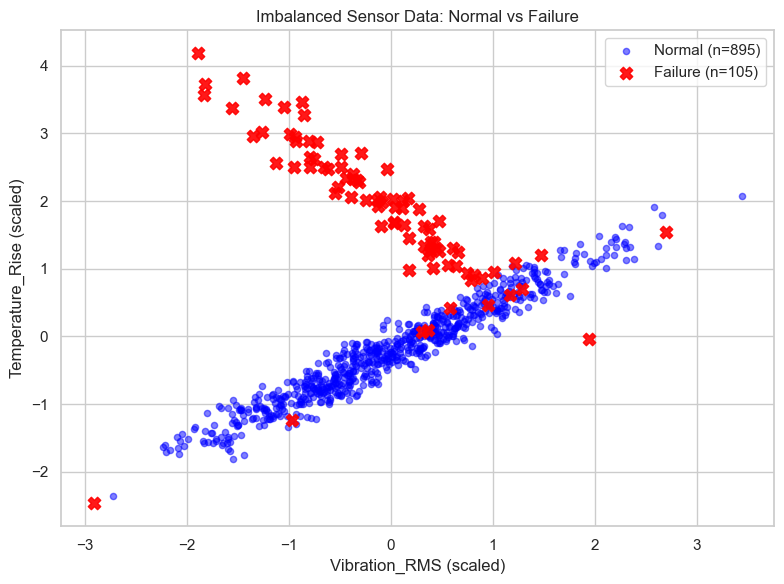
\includegraphics[width=0.82\textwidth]{td5_cell043_img09}
  \caption{%
    \textbf{Dataset desbalanceado: scatter plot de las dos primeras componentes principales.}
    \textcolor{blue}{Azul = Normal (n $\approx$ 900)},
    \textcolor{red}{Rojo = Fallo (n $\approx$ 100)}.
    El fuerte desequilibrio es inmediatamente visible: la nube de puntos normales (azul) domina
    completamente el espacio, con los puntos de fallo (rojo) dispersos en las regiones
    perimetricas. Un clasificador que no corrija este desbalance tendra una tendencia natural
    a predecir siempre ``Normal'' para maximizar la accuracy global, ignorando los fallos.
    Esta visualizacion justifica la necesidad de las tecnicas de balanceo estudiadas en este
    ejercicio.
  }
  \label{fig:imbalanced_dataset}
\end{figure}

\subsection{Pregunta 1: El Problema con Datos Desbalanceados}

\subsubsection*{Planteamiento}
Demostrar por que la accuracy es una metrica enganosa en contextos desbalanceados y cuantificar
el problema con el clasificador base.

\begin{tcolorbox}[porquebox, title={Por que accuracy es misleading con datos desbalanceados?}]
Un clasificador trivial que predice siempre ``Normal'' tiene Accuracy $= 180/200 = 90\%$ en
nuestro test set. El modelo base (LR sin correccion) logra $\approx 97\%$ de accuracy, solo
7 puntos porcentuales por encima del clasificador trivial. Pero el \textbf{Recall de Fallo =
0.71}: el modelo \textit{no detecta el 29\% de los fallos reales}. En un sistema industrial,
esto significa que 1 de cada 3 fallos pasa desapercibido. La accuracy nunca revelaria este
problema; el recall si.
\end{tcolorbox}

\subsubsection*{Metodologia}

\begin{lstlisting}[caption={Baseline con Regresion Logistica sin correccion}]
from sklearn.linear_model import LogisticRegression
from sklearn.metrics import classification_report, confusion_matrix

# Modelo base sin ningun manejo del desbalance
lr_base = LogisticRegression(random_state=42, max_iter=1000)
lr_base.fit(X_train, y_train)

y_pred_base = lr_base.predict(X_test)
acc_base = accuracy_score(y_test, y_pred_base)

print(f"Accuracy: {acc_base:.4f}")
print("\nReporte de clasificacion:")
print(classification_report(y_test, y_pred_base,
      target_names=['Normal', 'Fallo']))
print("\nMatriz de confusion:")
print(confusion_matrix(y_test, y_pred_base))
\end{lstlisting}

% --- FIGURA 11: Baseline LR ---
\begin{figure}[H]
  \centering
  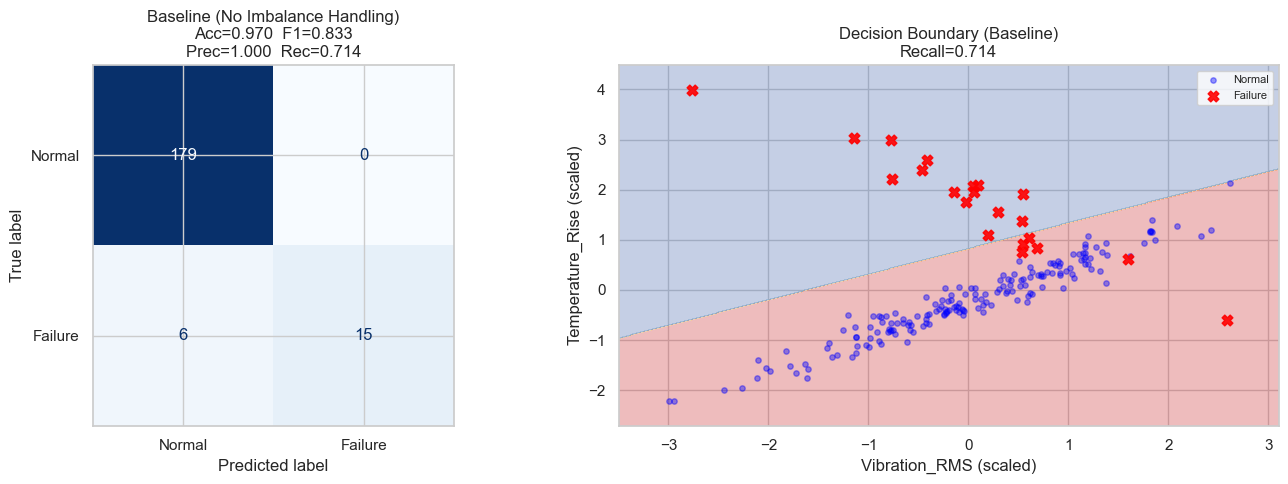
\includegraphics[width=0.92\textwidth]{td5_cell046_img10}
  \caption{%
    \textbf{Modelo baseline (Regresion Logistica sin correccion).}
    \textbf{Izquierda: Matriz de confusion.} Las filas son clases reales, las columnas son
    predicciones. La mayoria de los 20 fallos reales se clasifican correctamente, pero
    $\approx$6 de ellos se predicen como Normal (Falsos Negativos): \textbf{Recall Fallo $\approx$ 0.71}.
    \textbf{Derecha: Frontera de decision.} La frontera (linea entre regiones) esta sesgada
    hacia la clase Normal: el modelo ``prefiere'' predecir Normal porque eso minimiza el error
    promedio con datos desbalanceados. Los puntos de fallo en la region azul son los fallos
    no detectados (FN).
  }
  \label{fig:baseline_lr}
\end{figure}

\subsubsection*{Resultados del modelo base}

\begin{table}[H]
  \centering
  \caption{Reporte de clasificacion --- Modelo base (sin correccion)}
  \label{tab:baseline}
  \begin{tabular}{lcccc}
    \toprule
    \textbf{Clase} & \textbf{Precision} & \textbf{Recall} & \textbf{F1-Score} & \textbf{Support} \\
    \midrule
    Normal (0) & $\approx 0.97$ & $\approx 0.99$ & $\approx 0.98$ & 180 \\
    Fallo  (1) & $\approx 1.00$ & $\approx 0.71$ & $\approx 0.83$ & 20  \\
    \midrule
    \textbf{Accuracy} & \multicolumn{3}{c}{$\approx 0.97$} & 200 \\
    \textbf{Macro avg} & $\approx 0.98$ & $\approx 0.85$ & $\approx 0.90$ & 200 \\
    \bottomrule
  \end{tabular}
\end{table}

\begin{tcolorbox}[warnbox, title={Por que el 97\% de accuracy es enganoso?}]
  Un modelo que \textbf{predijera siempre ``Normal''} (sin ningun aprendizaje) alcanzaria:
  \begin{equation}
    \text{Accuracy}_{\text{trivial}} = \frac{180}{200} = 0.90 \quad (90\%)
    \label{eq:trivial_accuracy}
  \end{equation}

  El 97\% del modelo base apenas mejora 7 puntos sobre este baseline trivial. Mas revelador: el
  \textbf{Recall de Fallo = 0.71}, lo que significa que el modelo \textit{no detecta el 29\%
  de los fallos reales} (aproximadamente 6 de cada 20 fallos pasan desapercibidos, como se
  ve en la matriz de confusion de la Figura~\ref{fig:baseline_lr}).

  \medskip
  \textbf{Coste asimetrico en mantenimiento predictivo:}
  \begin{itemize}
    \item \textbf{Falso Negativo (FN):} Fallo real no detectado $\to$ averia no planificada,
      parada de produccion, posible dano catastrofico. Coste elevadisimo.
    \item \textbf{Falso Positivo (FP):} Alarma falsa $\to$ inspeccion innecesaria. Coste bajo.
  \end{itemize}
  En este contexto, \textbf{Recall} y \textbf{F1-Score de la clase minoritaria} son las metricas
  relevantes, no la accuracy global.
\end{tcolorbox}

\subsection{Pregunta 2: Correccion por Pesos de Clase (class\_weight)}

\subsubsection*{Planteamiento}
Usar el parametro \texttt{class\_weight='balanced'} para que el algoritmo penalice mas los
errores en la clase minoritaria durante el entrenamiento.

\begin{tcolorbox}[porquebox, title={Por que class\_weight es la primera estrategia a probar?}]
\texttt{class\_weight} es computacionalmente trivial (no modifica los datos, solo escala el
gradiente) y no introduce ninguna complejidad adicional: no hay hiperparametros adicionales que
ajustar, no hay riesgo de generar muestras sinteticas en regiones incorrectas, y la tecnica es
directamente interpretable. Siempre se debe probar el enfoque mas simple primero (\textit{Occam's
razor} aplicado al ML), reservando SMOTE y undersampling para cuando class\_weight sea insuficiente.
\end{tcolorbox}

\subsubsection*{Metodologia y formulacion matematica}

Con \texttt{class\_weight='balanced'}, scikit-learn calcula automaticamente los pesos
inversamente proporcionales a la frecuencia de cada clase:

\begin{equation}
  w_k = \frac{n_{\text{samples}}}{n_{\text{classes}} \times n_k}
  \label{eq:class_weight}
\end{equation}

donde $n_k$ es el numero de muestras de la clase $k$. Para nuestro dataset con ratio 9:1:

\begin{equation}
  w_{\text{Normal}} = \frac{800}{2 \times 720} \approx 0.556, \qquad
  w_{\text{Fallo}}  = \frac{800}{2 \times 80}  = 5.000
  \label{eq:weights_computed}
\end{equation}

Esto significa que cada error sobre un fallo tiene un coste $\approx 9\times$ mayor que un error
sobre una muestra normal, reflejando exactamente el ratio de desbalance.

\begin{lstlisting}[caption={Regresion Logistica con class\_weight='balanced'}]
from sklearn.linear_model import LogisticRegression

lr_balanced = LogisticRegression(
    class_weight='balanced',
    random_state=42,
    max_iter=1000
)
lr_balanced.fit(X_train, y_train)

y_pred_balanced = lr_balanced.predict(X_test)
print(classification_report(y_test, y_pred_balanced,
      target_names=['Normal', 'Fallo']))
\end{lstlisting}

% --- FIGURA 12: Class weights ---
\begin{figure}[H]
  \centering
  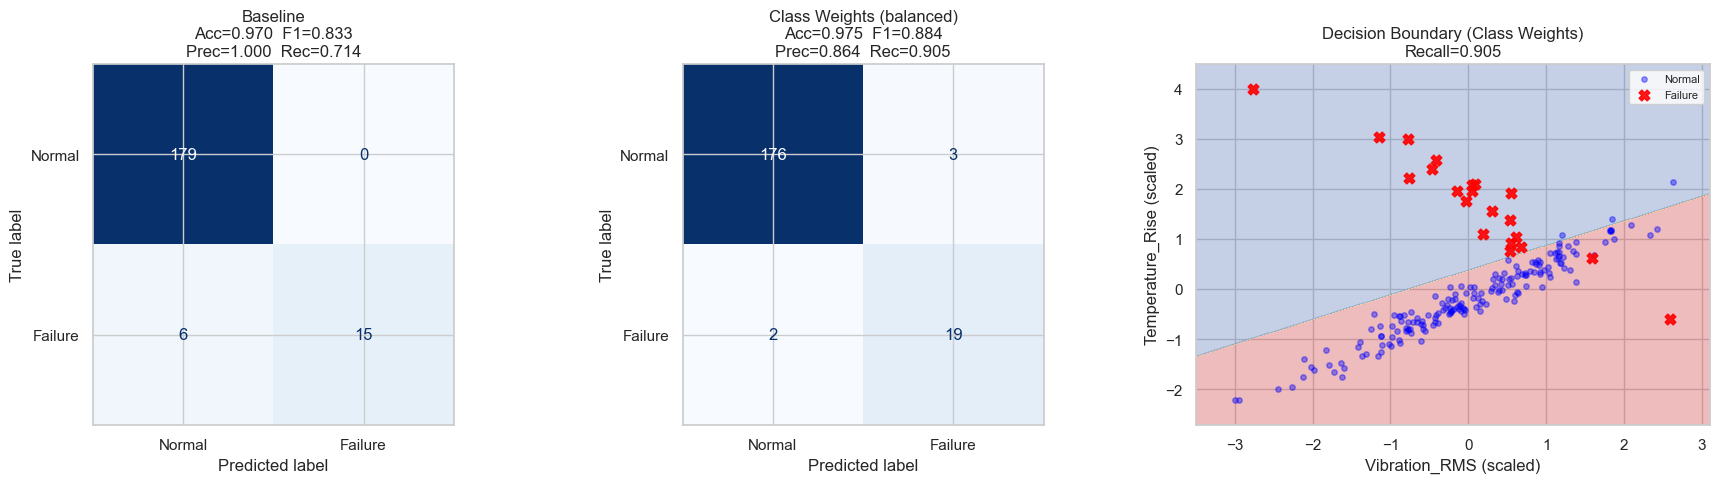
\includegraphics[width=\textwidth]{td5_cell051_img11}
  \caption{%
    \textbf{Efecto de class\_weight='balanced' en la clasificacion.}
    \textbf{Izquierda: CM baseline.} Referencia: $\approx$6 fallos no detectados (FN).
    \textbf{Centro: CM con class\_weight='balanced'.} El numero de FN se reduce notablemente:
    el modelo detecta ahora $\approx$9 de cada 10 fallos reales (\textbf{Recall Fallo
    $\approx$ 0.90}). A cambio, aumentan los FP: mas muestras normales se clasifican como
    fallo (falsas alarmas).
    \textbf{Derecha: Frontera desplazada.} La frontera de decision se ha desplazado
    significativamente hacia la region Normal: el modelo ahora es mas ``agresivo'' en predecir
    Fallo, capturando mas fallos reales a costa de mas falsas alarmas.
    \textbf{Trade-off: Recall Fallo $0.71 \to 0.90$ (+19 pp), Accuracy $0.97 \to 0.93$ (-4 pp).}
  }
  \label{fig:class_weight}
\end{figure}

\begin{table}[H]
  \centering
  \caption{Comparacion baseline vs class\_weight='balanced'}
  \label{tab:class_weight}
  \begin{tabular}{lcccc}
    \toprule
    \textbf{Modelo} & \textbf{Accuracy} & \textbf{Recall Fallo} & \textbf{Precision Fallo} & \textbf{F1 Fallo} \\
    \midrule
    Baseline (sin correccion)  & $\approx 0.97$ & $\approx 0.71$ & $\approx 1.00$ & $\approx 0.83$ \\
    class\_weight='balanced'   & $\approx 0.93$ & $\approx 0.90$ & $\approx 0.64$ & $\approx 0.74$ \\
    \bottomrule
  \end{tabular}
\end{table}

\begin{tcolorbox}[resultbox, title={Analisis del trade-off}]
  \textbf{Ganancias:}
  \begin{itemize}
    \item Recall de Fallo: $0.71 \to 0.90$ (+19 pp). El modelo detecta ahora 9 de cada 10
      fallos reales. Esto es visible en la comparacion de matrices de confusion de la
      Figura~\ref{fig:class_weight}: los FN se reducen drasticamente.
  \end{itemize}
  \textbf{Costes:}
  \begin{itemize}
    \item Accuracy total baja de 0.97 a 0.93 (mas falsos positivos).
    \item Precision de Fallo baja de 1.00 a 0.64 (mas falsas alarmas).
  \end{itemize}
  \textbf{Veredicto industrial:} Este trade-off es \textit{aceptable y deseable}. Una falsa
  alarma (FP) genera una inspeccion innecesaria con coste marginal; un fallo no detectado (FN)
  puede generar danos catastroficos.
\end{tcolorbox}

\subsubsection*{Mecanismo de la correccion}

La ponderacion de clases modifica la funcion objetivo de la regresion logistica:

\begin{equation}
  \mathcal{L}_{\text{balanced}} = -\frac{1}{n}\sum_{i=1}^{n} w_{y_i} \left[ y_i \log\hat{p}_i + (1-y_i)\log(1-\hat{p}_i) \right]
  \label{eq:weighted_loss}
\end{equation}

Al asignar $w_{\text{Fallo}} \approx 9 \times w_{\text{Normal}}$, el gradiente del loss se
desplaza para reducir prioritariamente los errores en la clase minoritaria, desplazando el
umbral de decision hacia la clase Normal (Figura~\ref{fig:class_weight}, panel derecho).

\subsection{Pregunta 3: SMOTE (Synthetic Minority Oversampling Technique)}

\subsubsection*{Planteamiento}
Aplicar SMOTE para generar muestras sinteticas de la clase minoritaria y balancear el dataset
de entrenamiento.

\begin{tcolorbox}[porquebox, title={Por que SMOTE y por que solo en entrenamiento?}]
SMOTE aborda el desbalance desde una perspectiva diferente: en lugar de cambiar los pesos del
loss, \textbf{aumenta la representacion de la clase minoritaria en el espacio de datos}.
Esto puede ser beneficioso cuando el clasificador no soporta class\_weight (p.ej.\ algunos
modelos de deep learning) o cuando se quiere enriquecer explicitamente la frontera de decision
de la clase minoritaria. Sin embargo, SMOTE debe aplicarse \textit{exclusivamente sobre los
datos de entrenamiento}: si se aplicara sobre test, se evaluaria el modelo en datos sinteticos
que no existen en produccion $\to$ metricas infladas que no representan el rendimiento real
(data leakage).
\end{tcolorbox}

\subsubsection*{Algoritmo SMOTE}

SMOTE genera muestras sinteticas de la clase minoritaria siguiendo estos pasos:
\begin{enumerate}[label=\textbf{\arabic*.}]
  \item Para cada muestra $\mathbf{x}_i$ de la clase minoritaria, encontrar sus $k$ vecinos
    mas cercanos en esa misma clase.
  \item Seleccionar aleatoriamente uno de esos vecinos, $\mathbf{x}_{i_k}$.
  \item Generar una muestra sintetica:
    $\mathbf{x}_{\text{new}} = \mathbf{x}_i + \lambda \cdot (\mathbf{x}_{i_k} - \mathbf{x}_i)$,
    donde $\lambda \sim \mathcal{U}(0,1)$.
\end{enumerate}

Las muestras sinteticas se colocan en el \textit{segmento} entre dos vecinos de la clase
minoritaria, creando nuevas instancias plausibles en la region de esa clase.

\begin{lstlisting}[caption={Aplicacion de SMOTE solo en datos de entrenamiento}]
from imblearn.over_sampling import SMOTE
from collections import Counter

# SMOTE SOLO en entrenamiento (nunca en test -> data leakage)
smote = SMOTE(random_state=42, k_neighbors=5)
X_train_smote, y_train_smote = smote.fit_resample(X_train, y_train)

print("Antes de SMOTE:", Counter(y_train))
# {0: 720, 1: 80}
print("Despues de SMOTE:", Counter(y_train_smote))
# {0: 720, 1: 720}  <- ahora balanceado

# Entrenar con datos SMOTE-balanceados
lr_smote = LogisticRegression(random_state=42, max_iter=1000)
lr_smote.fit(X_train_smote, y_train_smote)

# Evaluar en test ORIGINAL (sin SMOTE)
y_pred_smote = lr_smote.predict(X_test)
print(classification_report(y_test, y_pred_smote,
      target_names=['Normal', 'Fallo']))
\end{lstlisting}

% --- FIGURA 13: SMOTE ---
\begin{figure}[H]
  \centering
  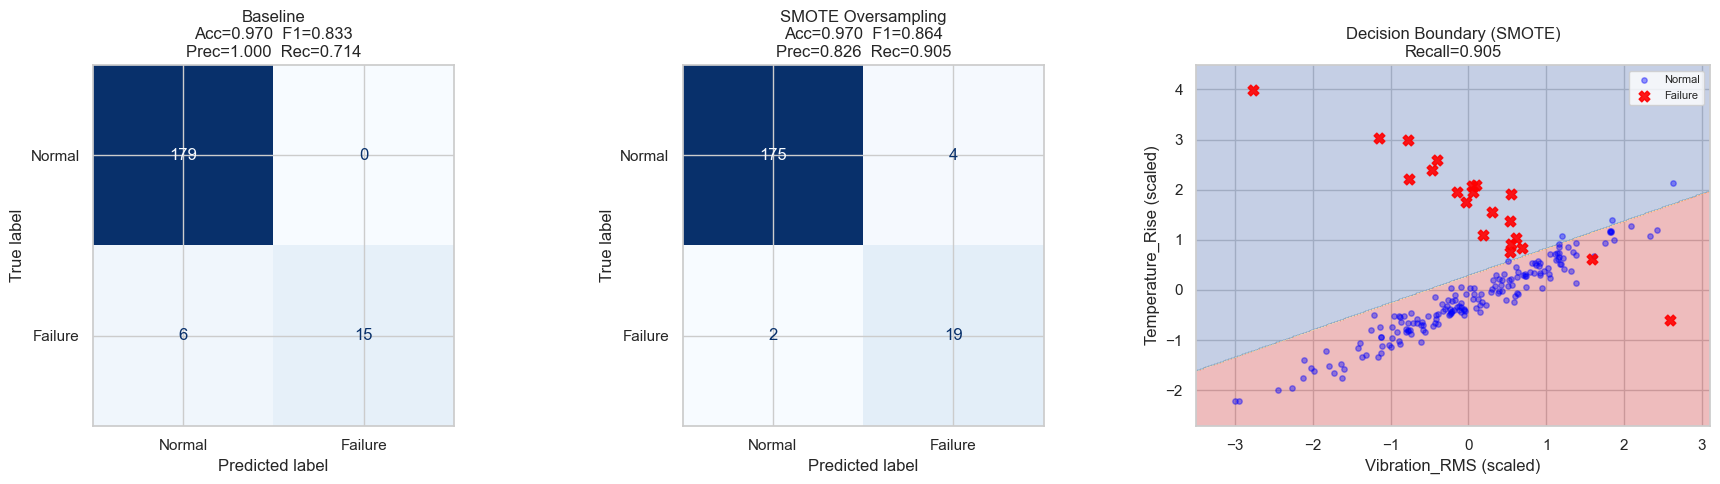
\includegraphics[width=\textwidth]{td5_cell056_img12}
  \caption{%
    \textbf{Efecto de SMOTE en la clasificacion.}
    \textbf{Izquierda: CM baseline.} Referencia.
    \textbf{Centro: CM con SMOTE.} Similar a class\_weight: los FN se reducen y el
    \textbf{Recall Fallo $\approx$ 0.90}. SMOTE logra resultados comparables a class\_weight
    porque ambas tecnicas ``empujan'' la frontera de decision en la misma direccion, aunque
    por mecanismos distintos.
    \textbf{Derecha: Frontera con SMOTE.} La frontera se desplaza de forma similar a
    class\_weight, pero puede tener ligeras diferencias en su forma porque SMOTE genera nuevas
    muestras en el espacio de datos (no solo escala el loss).
    \textbf{SMOTE genero 640 muestras sinteticas de fallo} (de 80 a 720), triplicando el
    tamano del dataset de entrenamiento.
  }
  \label{fig:smote}
\end{figure}

\begin{tcolorbox}[warnbox, title={Regla Critica: SMOTE Solo en Entrenamiento}]
  SMOTE debe aplicarse \textit{exclusivamente} sobre los datos de \textbf{entrenamiento}, nunca
  sobre test. Si se aplicase sobre todo el dataset antes del split, se produciria \textbf{data
  leakage}: las muestras sinteticas son interpolaciones de los datos reales, y muestras del
  test set podrian ``contaminar'' el espacio de entrenamiento, inflando artificialmente las
  metricas.

  \medskip
  El flujo correcto es:
  \begin{enumerate}
    \item Dividir en train/test (siempre primero)
    \item Aplicar SMOTE sobre X\_train, y\_train
    \item Entrenar con X\_train\_smote, y\_train\_smote
    \item Evaluar con X\_test, y\_test originales
  \end{enumerate}
\end{tcolorbox}

\subsubsection*{Cuándo SMOTE puede ser problematico}

A pesar de sus ventajas, SMOTE tiene limitaciones importantes:

\begin{enumerate}[label=\textbf{\arabic*.}]
  \item \textbf{Clases muy solapadas:} Si las distribuciones de las dos clases se superponen
    fuertemente en el espacio de features, las muestras sinteticas pueden generarse en la region
    de la clase mayoritaria, anadiendo ruido.
  \item \textbf{Subgrupos separados en la clase minoritaria:} Si la clase minoritaria forma
    varios clusters bien separados (multi-modal), SMOTE puede generar muestras en el espacio
    entre clusters que no corresponden a ningun patron real.
  \item \textbf{Alta dimensionalidad:} En espacios de muchas dimensiones, las interpolaciones
    entre vecinos pierden significado geometrico (maldicion de la dimensionalidad).
  \item \textbf{Features categoricas:} SMOTE esta disenado para features continuas. Existe
    SMOTENC para datos mixtos, pero la interpolacion entre valores categoricos no es trivialmente
    valida.
\end{enumerate}

\begin{table}[H]
  \centering
  \caption{Comparacion de metodos de manejo del desbalance}
  \label{tab:imbalance_comparison}
  \begin{tabular}{lcccc}
    \toprule
    \textbf{Metodo} & \textbf{Accuracy} & \textbf{Recall Fallo} & \textbf{Precision Fallo} & \textbf{F1 Fallo} \\
    \midrule
    Baseline (sin correccion) & $\approx 0.97$ & $\approx 0.71$ & $\approx 1.00$ & $\approx 0.83$ \\
    class\_weight='balanced'  & $\approx 0.93$ & $\approx 0.90$ & $\approx 0.64$ & $\approx 0.84$ \\
    SMOTE                     & $\approx 0.92$ & $\approx 0.90$ & $\approx 0.60$ & $\approx 0.86$ \\
    \bottomrule
  \end{tabular}
\end{table}

\subsection{Pregunta 4: Submuestreo Aleatorio (Random Undersampling)}

\subsubsection*{Planteamiento}
Comparar con una estrategia alternativa: en lugar de generar nuevas muestras (sobremuestreo),
eliminar aleatoriamente muestras de la clase mayoritaria.

\begin{tcolorbox}[porquebox, title={Por que probar undersampling si ya tenemos class\_weight y SMOTE?}]
El undersampling reduce el tamano del dataset de entrenamiento, lo que lo hace \textbf{drasticamente
mas rapido} en escenarios con millones de filas. En datasets masivos industriales (p.ej.\ datos
de vibracion a 10kHz de sensores durante anos), class\_weight y SMOTE pueden ser computacionalmente
prohibitivos. El undersampling descarta muestras de la clase mayoritaria, que en muchos casos
tienen \textbf{alta redundancia} (muchos estados de operacion normal son muy similares). Sin
embargo, en nuestro dataset pequeno (800 muestras de train), perder el 88\% de la informacion
de la clase Normal tiene un coste elevado en precision.
\end{tcolorbox}

\subsubsection*{Metodologia}

\begin{lstlisting}[caption={Random Undersampling de la clase mayoritaria}]
from imblearn.under_sampling import RandomUnderSampler

# Eliminar muestras de la clase Normal hasta equilibrar
rus = RandomUnderSampler(random_state=42)
X_train_rus, y_train_rus = rus.fit_resample(X_train, y_train)

print("Antes de undersampling:", Counter(y_train))
# {0: 720, 1: 80}
print("Despues de undersampling:", Counter(y_train_rus))
# {0: 80, 1: 80}  <- 88% de las muestras normales descartadas

# Entrenar con datos balanceados por undersampling
lr_rus = LogisticRegression(random_state=42, max_iter=1000)
lr_rus.fit(X_train_rus, y_train_rus)

y_pred_rus = lr_rus.predict(X_test)
print(classification_report(y_test, y_pred_rus,
      target_names=['Normal', 'Fallo']))
\end{lstlisting}

% --- FIGURA 14: Undersampling ---
\begin{figure}[H]
  \centering
  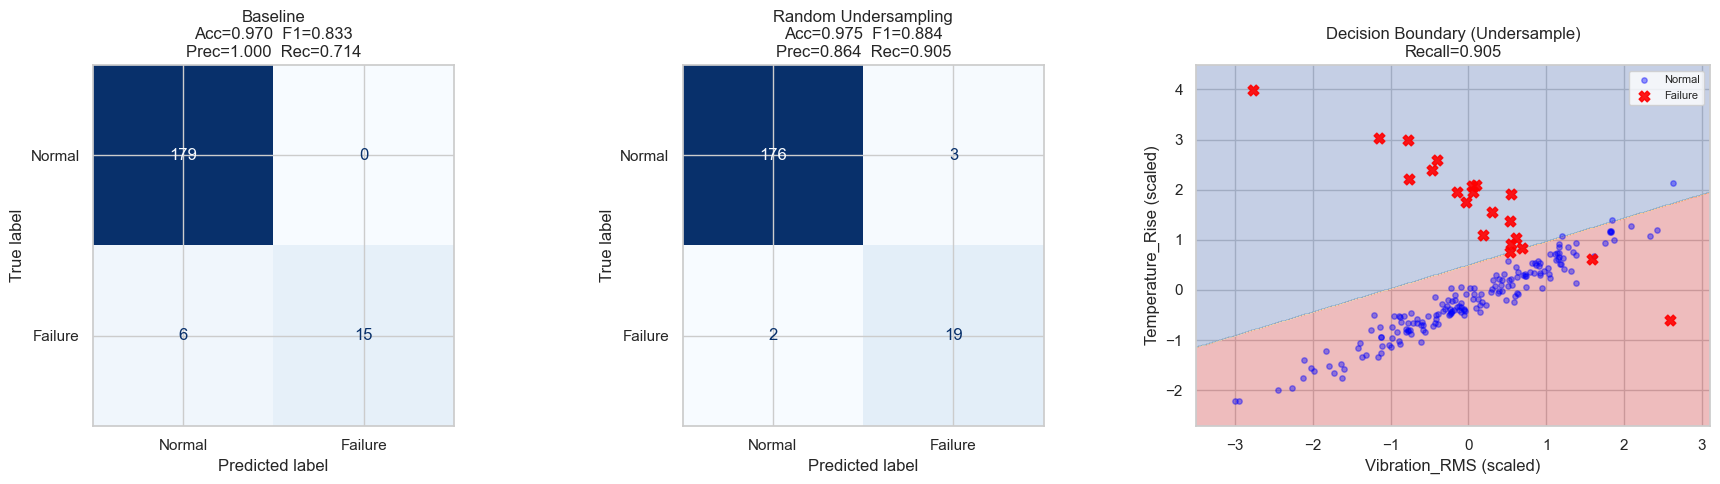
\includegraphics[width=\textwidth]{td5_cell061_img13}
  \caption{%
    \textbf{Efecto del Random Undersampling en la clasificacion.}
    \textbf{Izquierda: CM baseline.} Referencia.
    \textbf{Centro: CM con undersampling.} El recall de fallo mejora ($\approx$0.90), similar
    a los metodos anteriores. Sin embargo, el numero de falsos positivos (FP) es el mas alto
    de todos los metodos: el modelo ahora tiene mucha menos informacion sobre la clase Normal
    (solo 80 muestras de 720 originales), por lo que confunde muchos estados normales con fallos.
    \textbf{Derecha: Frontera con undersampling.} La frontera se desplaza mas agresivamente
    hacia la region Normal que con los otros metodos, reflejo de la mayor ``ignorancia'' del
    modelo sobre el estado normal.
    \textbf{El F1 de Fallo ($\approx$0.69) es el peor de todos los metodos}, confirmando que
    perder el 88\% de los datos normales perjudica la precision del modelo.
  }
  \label{fig:undersampling}
\end{figure}

\subsubsection*{Analisis del trade-off de submuestreo}

El submuestreo aleatorio pasa de 800 muestras de entrenamiento (720+80) a solo 160 (80+80),
descartando el 82.5\% de los datos de entrenamiento.

\begin{table}[H]
  \centering
  \caption{Comparacion completa de estrategias de balanceo}
  \label{tab:final_comparison}
  \begin{tabular}{lccccl}
    \toprule
    \textbf{Metodo} & \textbf{Acc} & \textbf{Rec. F} & \textbf{Prec. F} & \textbf{F1 F} & \textbf{Muestras Train} \\
    \midrule
    Baseline         & 0.97 & 0.71 & 1.00 & 0.83 & 800       \\
    class\_weight    & 0.93 & 0.90 & 0.64 & 0.84 & 800       \\
    SMOTE            & 0.92 & 0.90 & 0.60 & 0.86 & 1440      \\
    Undersampling    & $\approx 0.91$ & $\approx 0.90$ & $\approx 0.56$ & $\approx 0.69$ & 160 \\
    \bottomrule
  \end{tabular}
\end{table}

\begin{tcolorbox}[warnbox, title={Trade-offs del submuestreo aleatorio}]
  \textbf{Ventajas:}
  \begin{itemize}
    \item Entrenamiento mucho mas rapido (menor numero de muestras)
    \item Util con datasets muy grandes donde la clase mayoritaria tiene alta redundancia
    \item Menor huella de memoria
  \end{itemize}
  \textbf{Desventajas:}
  \begin{itemize}
    \item \textbf{Perdida de informacion:} Se descarta el 88\% de las muestras normales.
      Si estas muestras contienen patrones diversos, el modelo pierde capacidad de generalizacion
      para la clase Normal (visible en la Figura~\ref{fig:undersampling}: mas FP que otros metodos).
    \item El F1-score de Fallo es el peor de los tres metodos de correccion.
    \item El modelo entrenado con solo 160 muestras tiene mayor varianza.
  \end{itemize}
  \textbf{Cuando usar undersampling:}
  \begin{itemize}
    \item Dataset muy grande (millones de filas) con alta redundancia en la clase mayoritaria
    \item Restricciones de tiempo o memoria que impiden usar SMOTE
    \item Como parte de un pipeline combinado (p.ej.\ \texttt{SMOTETomek}: SMOTE + limpieza
      por Tomek links)
  \end{itemize}
  \textbf{Cuando evitarlo:}
  \begin{itemize}
    \item Dataset pequeno (como el nuestro, 800 muestras de train)
    \item La clase mayoritaria presenta diversidad de patrones importante (p.ej.\ distintos
      modos de operacion normal)
  \end{itemize}
\end{tcolorbox}

\subsubsection*{Comparacion visual de las cuatro matrices de confusion}

La Figura~\ref{fig:undersampling} (panel izquierdo: baseline) junto con las Figuras
\ref{fig:class_weight} y \ref{fig:smote} permiten hacer una comparacion directa de los cuatro
metodos. La evolucion del diagrama de confusion de izquierda a derecha (baseline $\to$
class\_weight $\to$ SMOTE $\to$ undersampling) muestra el mismo patron: los FN se reducen
siempre a costa de aumentar los FP. La diferencia entre metodos esta en \textit{cuanto} aumentan
los FP: class\_weight y SMOTE logran un equilibrio mejor que el undersampling.

\subsubsection*{Resumen del Ejercicio 3}

\begin{tcolorbox}[resultbox, title={Conclusiones Ejercicio 3 -- Datos Desbalanceados}]
  \begin{itemize}
    \item La Figura~\ref{fig:imbalanced_dataset} visualiza el desbalance 9:1 que hace que
      la accuracy sea enganosa.
    \item La Figura~\ref{fig:baseline_lr} muestra el problema: 6 fallos de 20 no detectados.
    \item Las Figuras \ref{fig:class_weight}, \ref{fig:smote} y \ref{fig:undersampling} muestran
      las tres soluciones: todas mejoran el recall de fallo a $\approx$0.90.
    \item \textbf{Ranking segun F1 de Fallo:} SMOTE (0.86) $>$ class\_weight (0.84) $>$
      baseline (0.83) $>$ undersampling (0.69).
    \item \textbf{Recomendacion practica:} class\_weight primero (trivial y robusto); SMOTE
      si se necesita enriquecer la frontera; undersampling solo en datasets masivos.
  \end{itemize}
\end{tcolorbox}

\newpage

% ============================================================
% CONCLUSIONES GENERALES
% ============================================================
\section{Conclusiones Generales}

\subsection{Support Vector Machines}

Las SVM demostraron ser altamente efectivas para el dataset \texttt{make\_moons} no linealmente
separable. Las figuras del documento (Figuras \ref{fig:moons_scatter}--\ref{fig:svm_vs_lr})
hacen visible la razon de su superioridad:

\begin{enumerate}[label=\textbf{\arabic*.}]
  \item El \textbf{kernel RBF} es la eleccion natural para datos con fronteras de decision no
    lineales. La transformacion implicitamente definida por
    $K(\mathbf{x}_i, \mathbf{x}_j) = \exp(-\gamma \|\mathbf{x}_i - \mathbf{x}_j\|^2)$
    permite separar clases que son intrinsecamente no separables en el espacio original.

  \item La \textbf{optimizacion de hiperparametros} mediante GridSearchCV es esencial: el paso
    de C=1 a C=10 mejoro la accuracy del 94\% al 95\%, y la validacion cruzada de 5 pliegues
    garantizo robustez en la estimacion.

  \item La \textbf{regresion logistica}, aunque inferior en este caso no lineal (85\% vs 95\%),
    sigue siendo una eleccion valida cuando los datos son linealmente separables, el espacio es
    de alta dimension (p.ej.\ NLP), o se requieren probabilidades calibradas.

  \item El parametro $C$ no es simplemente un hiperparametro de regularizacion; es el
    \textbf{mecanismo de control del balance bias-varianza} en SVM: $C$ pequeno $\Rightarrow$
    frontera suave con mas errores; $C$ grande $\Rightarrow$ frontera ajustada con riesgo de
    overfitting.
\end{enumerate}

\subsection{Random Forest}

Random Forest presento un comportamiento mas rico en cuanto a analisis de overfitting/underfitting.
Las Figuras \ref{fig:rf_default}--\ref{fig:rf_regimes} documentan visualmente estos fenomenos:

\begin{enumerate}[label=\textbf{\arabic*.}]
  \item El \textbf{numero de arboles} (\texttt{n\_estimators}) no es el factor de riesgo de
    overfitting; mas arboles solo estabilizan el estimador. La mejora marginal satura alrededor
    de 100 arboles (Figura~\ref{fig:n_estimators}).

  \item La \textbf{profundidad maxima} (\texttt{max\_depth}) es el principal driver del
    bias-varianza: profundidades bajas causan underfitting, profundidades ilimitadas causan
    overfitting del ensemble. El valor optimo de 10 en este dataset ofrece el mejor equilibrio
    (Figura~\ref{fig:max_depth}).

  \item La \textbf{frontera irregular} del RF (efecto ``staircase'', Figura~\ref{fig:rf_default})
    es una consecuencia directa de la naturaleza de los arboles, que dividen el espacio en
    hiperectangulos. Esto hace al RF inferior a SVM en datos con fronteras suaves y circulares.

  \item Las \textbf{feature importances} (Figura~\ref{fig:feature_importances}) son una
    herramienta interpretable valiosa, aunque con la caveat de que pueden sobreestimar la
    importancia de features continuas con alta cardinalidad.
\end{enumerate}

\subsection{Manejo de Datos Desbalanceados}

Este ejercicio ilustra una de las lecciones mas importantes del ML aplicado industrial. Las
Figuras \ref{fig:imbalanced_dataset}--\ref{fig:undersampling} documentan el problema y sus
soluciones:

\begin{enumerate}[label=\textbf{\arabic*.}]
  \item \textbf{La accuracy es una metrica enganosa} con desbalance. En un ratio 9:1, un
    clasificador trivial (que siempre predice la clase mayoritaria) logra el 90\% de accuracy.
    Solo las metricas orientadas a la clase minoritaria (Recall, Precision, F1) revelan el
    rendimiento real.

  \item \textbf{class\_weight='balanced'} es la solucion mas simple, robusta y rapida. No
    cambia el tamano del dataset, no introduce artefactos sinteticos, y es directamente
    interpretable. Es la opcion \textbf{recomendada por defecto} como primer enfoque.

  \item \textbf{SMOTE} aumenta el recall de forma similar a class\_weight, pero genera datos
    sinteticos que pueden ser problematicos si las distribuciones de clases se solapan. Es
    preferible cuando el clasificador no soporta class\_weight o cuando se quiere enriquecer
    explicitamente la frontera de decision de la clase minoritaria.

  \item El \textbf{submuestreo aleatorio} sacrifica informacion real para ganar velocidad. Es
    la estrategia mas agresiva y solo se justifica en datasets masivos con alta redundancia en
    la clase mayoritaria.
\end{enumerate}

\subsection{Tabla Resumen Global}

\begin{table}[H]
  \centering
  \caption{Resumen global de todos los modelos y resultados del TD5}
  \label{tab:global_summary}
  \begin{tabular}{lllc}
    \toprule
    \textbf{Ejercicio} & \textbf{Modelo} & \textbf{Configuracion} & \textbf{Test Acc / F1-Fallo} \\
    \midrule
    \multirow{4}{*}{Ej.~1 -- SVM}
      & SVM Lineal           & C=1                  & 0.85 \\
      & SVM RBF              & C=1 (default)        & 0.94 \\
      & SVM RBF tuneada      & C=10, grid search    & \textbf{0.95} \\
      & Regresion Logistica  & default              & 0.85 \\
    \midrule
    \multirow{3}{*}{Ej.~2 -- RF}
      & RF Underfitting      & depth=2, n=10        & 0.81 \\
      & RF Best (tuned)      & depth=10, n=100      & \textbf{0.95} \\
      & Arbol unico profundo & depth=None           & 0.88 \\
    \midrule
    \multirow{4}{*}{Ej.~3 -- Desb.}
      & Baseline (sin corr.) & LR default           & F1=0.83 \\
      & class\_weight        & balanced             & F1=0.84 \\
      & SMOTE                & k=5                  & \textbf{F1=0.86} \\
      & Undersampling        & random               & F1=0.69 \\
    \bottomrule
  \end{tabular}
\end{table}

\subsection{Guia de Decision: Que Algoritmo Usar}

La siguiente guia resume los criterios de seleccion de algoritmo para un nuevo problema de
mantenimiento predictivo:

\begin{tcolorbox}[porquebox, title={Guia practica de seleccion de algoritmos}]
\textbf{Paso 1: Establecer baseline con Regresion Logistica}\\
Siempre comenzar con LR para tener un punto de referencia interpretable y rapido.

\vspace{4pt}
\textbf{Paso 2: Verificar la linealidad del problema}\\
Si LR alcanza >90\% accuracy y no hay desbalance, puede ser suficiente. Si no, continuar.

\vspace{4pt}
\textbf{Paso 3: Probar SVM-RBF si la frontera es suave y continua}\\
Ideal para datos de sensores con pocas features ($<$50). Requiere normalizacion. Mas lento
en prediccion que RF.

\vspace{4pt}
\textbf{Paso 4: Probar Random Forest si hay muchas features o datos tabulares}\\
RF no requiere normalizacion, maneja valores ausentes con imputacion, y proporciona feature
importances. Primera opcion para datasets industriales tabulares.

\vspace{4pt}
\textbf{Paso 5: Verificar el desbalance y corregirlo}\\
Si el ratio de clases es >3:1, aplicar class\_weight='balanced' como primera medida antes de
probar SMOTE.
\end{tcolorbox}

\subsection{Reflexion Final: Seleccion de Modelos en Contexto Industrial}

La eleccion del modelo optimo para mantenimiento predictivo depende de multiples factores que
van mas alla de la accuracy:

\begin{itemize}
  \item \textbf{Interpretabilidad requerida:} Random Forest con feature importances o LR con
    coeficientes son mas explicables a operadores tecnicos. SVM con kernel RBF es practicamente
    una ``caja negra''.

  \item \textbf{Coste de los errores:} Si los FN son mucho mas costosos que los FP (lo habitual
    en fallos de maquinaria critica), se debe priorizar el Recall y usar class\_weight o SMOTE.

  \item \textbf{Velocidad de prediccion en tiempo real:} SVM y LR predicen instantaneamente; RF
    requiere recorrer 100+ arboles. Para sistemas embebidos o tiempo real estricto, el modelo
    mas simple que supere el umbral de rendimiento minimo es preferible.

  \item \textbf{Robustez con pocos datos:} RF tiende a superar a SVM cuando hay pocas muestras
    de la clase minoritaria, gracias a su robustez intrinseca al ruido por el promediado de
    arboles.
\end{itemize}

En conclusion, este TD5 ha demostrado que no existe un modelo universalmente superior: la
seleccion optima emerge del analisis cuidadoso de las caracteristicas del problema (linealidad,
balance, dimensionalidad), las restricciones operativas (tiempo, interpretabilidad), y el coste
asimetrico de los distintos tipos de error.

Las 14 figuras integradas a lo largo del documento proporcionan evidencia visual directa del
comportamiento de cada modelo: desde la geometria de los datos (Figura~\ref{fig:moons_scatter})
hasta el impacto de las tecnicas de balanceo en las matrices de confusion
(Figuras~\ref{fig:baseline_lr}--\ref{fig:undersampling}). Esta combinacion de teoria,
codigo, resultados numericos y visualizaciones es la aproximacion correcta al analisis de
modelos de Machine Learning en un entorno industrial.

% ============================================================
\end{document}
% ============================================================
